\documentclass[]{book}
\usepackage{lmodern}
\usepackage{amssymb,amsmath}
\usepackage{ifxetex,ifluatex}
\usepackage{fixltx2e} % provides \textsubscript
\ifnum 0\ifxetex 1\fi\ifluatex 1\fi=0 % if pdftex
  \usepackage[T1]{fontenc}
  \usepackage[utf8]{inputenc}
\else % if luatex or xelatex
  \ifxetex
    \usepackage{mathspec}
  \else
    \usepackage{fontspec}
  \fi
  \defaultfontfeatures{Ligatures=TeX,Scale=MatchLowercase}
\fi
% use upquote if available, for straight quotes in verbatim environments
\IfFileExists{upquote.sty}{\usepackage{upquote}}{}
% use microtype if available
\IfFileExists{microtype.sty}{%
\usepackage{microtype}
\UseMicrotypeSet[protrusion]{basicmath} % disable protrusion for tt fonts
}{}
\usepackage[margin=1in]{geometry}
\usepackage{hyperref}
\hypersetup{unicode=true,
            pdftitle={Stat 850 Final Exam},
            pdfauthor={Dani Chu},
            pdfborder={0 0 0},
            breaklinks=true}
\urlstyle{same}  % don't use monospace font for urls
\usepackage{natbib}
\bibliographystyle{apalike}
\usepackage{longtable,booktabs}
\usepackage{graphicx,grffile}
\makeatletter
\def\maxwidth{\ifdim\Gin@nat@width>\linewidth\linewidth\else\Gin@nat@width\fi}
\def\maxheight{\ifdim\Gin@nat@height>\textheight\textheight\else\Gin@nat@height\fi}
\makeatother
% Scale images if necessary, so that they will not overflow the page
% margins by default, and it is still possible to overwrite the defaults
% using explicit options in \includegraphics[width, height, ...]{}
\setkeys{Gin}{width=\maxwidth,height=\maxheight,keepaspectratio}
\IfFileExists{parskip.sty}{%
\usepackage{parskip}
}{% else
\setlength{\parindent}{0pt}
\setlength{\parskip}{6pt plus 2pt minus 1pt}
}
\setlength{\emergencystretch}{3em}  % prevent overfull lines
\providecommand{\tightlist}{%
  \setlength{\itemsep}{0pt}\setlength{\parskip}{0pt}}
\setcounter{secnumdepth}{5}
% Redefines (sub)paragraphs to behave more like sections
\ifx\paragraph\undefined\else
\let\oldparagraph\paragraph
\renewcommand{\paragraph}[1]{\oldparagraph{#1}\mbox{}}
\fi
\ifx\subparagraph\undefined\else
\let\oldsubparagraph\subparagraph
\renewcommand{\subparagraph}[1]{\oldsubparagraph{#1}\mbox{}}
\fi

%%% Use protect on footnotes to avoid problems with footnotes in titles
\let\rmarkdownfootnote\footnote%
\def\footnote{\protect\rmarkdownfootnote}

%%% Change title format to be more compact
\usepackage{titling}

% Create subtitle command for use in maketitle
\newcommand{\subtitle}[1]{
  \posttitle{
    \begin{center}\large#1\end{center}
    }
}

\setlength{\droptitle}{-2em}

  \title{Stat 850 Final Exam}
    \pretitle{\vspace{\droptitle}\centering\huge}
  \posttitle{\par}
    \author{Dani Chu}
    \preauthor{\centering\large\emph}
  \postauthor{\par}
    \date{}
    \predate{}\postdate{}
  
\usepackage{booktabs}

\begin{document}
\maketitle

{
\setcounter{tocdepth}{1}
\tableofcontents
}
\hypertarget{question-1}{%
\chapter{Question 1}\label{question-1}}

\hypertarget{part-a}{%
\section{Part A}\label{part-a}}

Prove that the quadratic form \(y^{T} A y\), \(y^{T} B y\) are independent iff \(B \Sigma A = 0\).

We know that if a symmetric matrix \(A\) is of full rank then it can be written \(A = LL^T\) where \(L\) has full column rank

\begin{align}
  B \Sigma A &= 0 \\
  L_{B}L_{B}^T \Sigma L_{A}L_{A}^T & = 0
\end{align}

\hypertarget{part-b}{%
\section{Part B}\label{part-b}}

Let's start by rearranging \(R\).

\begin{align}
  R =& (K^T \hat{\beta} -m )^T (K^T (X^T X)^{-1} K)^{-1} (K^T \hat{\beta} - m) \\
    =& (K^T (X^T X)^{-1} X^T y - m )^T (K^T (X^T X)^{-1} K)^{-1} (K^T (X^T X)^{-1} X^T y - m) \\
    =& [ (K^T (X^T X)^{-1} X^T ) ( y - X K (K^T K)^{-1} m ) ]^T [ (K^T (X^T X)^{-1} K)^{-1} ] \\
    & [ (K^T (X^T X)^{-1} X^T ( y - X K (K^T K)^{-1} m ) ] \\
    =& [ ( y - X K (K^T K)^{-1} m ) ]^T [ X^T (X^T X)^{-1} K ] [ (K^T (X^T X)^{-1} K)^{-1} ] \\
    & [ (K^T (X^T X)^{-1} X^T] [( y - X K (K^T K)^{-1} m ) ] \\
    =& [y_{\text{new}}]^T A [y_{\text{new}}]
\end{align}

where

\begin{align}
  y_{\text{new}} = ( y - X K (K^T K)^{-1} m )
\end{align}

and

\begin{align}
  A = [ X^T (X^T X)^{-1} K ] [ (K^T (X^T X)^{-1} K)^{-1} ] [ (K^T (X^T X)^{-1} X^T]
\end{align}

Now to use the therorem we need to have \(SSE = y^T (I-H) y\) to be equal to \(y_{\text{new}}^T (I-H) y_{\text{new}}\).

\begin{align}
  y_{\text{new}}^T (I-H) y_{\text{new}} =& ( y - X K (K^T K)^{-1} m )^T (I-H) ( y - X K (K^T K)^{-1} m ) \\
  y_{\text{new}}^T (I-H) y_{\text{new}} =& ( y^T - m^T(K^T K)^{-1} K^T x^T ) (I-H) ( y - X K (K^T K)^{-1} m ) \\
  y_{\text{new}}^T (I-H) y_{\text{new}} =& y^T (I-H) y + \\
  & y^T (I-H) (- X K (K^T K)^{-1} m )) + \\
  & (-m^T(K^T K)^{-1} K^T x^T ) (I-H) ( y ) + \\
  & (-m^T(K^T K)^{-1} K^T x^T ) (I-H)(- X K (K^T K)^{-1} m ))\\
  y_{\text{new}}^T (I-H) y_{\text{new}} =& y^T (I-H) y + 0 + 0 + 0\\
   y_{\text{new}}^T (I-H) y_{\text{new}} =& y^T (I-H) y
\end{align}

So let

\begin{align}
  B = (I - H)
\end{align}

Finally let \(\Sigma = \sigma^2 I\) then

\begin{align}
  B \Sigma A &= (I - H) \sigma^2 I [ X^T (X^T X)^{-1} K ] [ (K^T (X^T X)^{-1} K)^{-1} ] [ (K^T (X^T X)^{-1} X^T]
  B \Sigma A &= 0
\end{align}

and we have set up the problem to use the theororem from part a. Therefore SSE and R under the genreal linear hypthesis are independent.

\hypertarget{part-c}{%
\section{Part C}\label{part-c}}

At the end of lecture 4 we have

\begin{align}
  \frac{R/\sigma^2 s}{SSE/ (\sigma^2 (n - (p + 1)) )} \sim F
\end{align}

We also know that the quotient of independently distributed chi-squared variables that have been divided by their degrees of freedom follows an F distribution. Both \(R\) and \(SSE\) have a chi-square distribution since they are sums of quadratic normals.

\hypertarget{part-d}{%
\section{Part D}\label{part-d}}

\hypertarget{question-2}{%
\chapter{Question 2}\label{question-2}}

\hypertarget{part-a-1}{%
\section{Part A}\label{part-a-1}}

I fit a multiple linear regression model to the data given in the file ``question2.txt''. The estimated least squares regression coefficients are presented in table \ref{tab:coefs}.

\begin{table}

\caption{\label{tab:coefs}OLS regression coefficients}
\centering
\begin{tabular}[t]{lr}
\toprule
Term & Estimate\\
\midrule
Intercept & 0.02\\
Regressor 1 & 0.81\\
Regressor 2 & 1.89\\
Regressor 3 & -3.01\\
Regressor 4 & -4.21\\
Regressor 5 & -4.71\\
\bottomrule
\end{tabular}
\end{table}

\hypertarget{part-b-1}{%
\section{Part B}\label{part-b-1}}

For the model fit in part A, the estimate for \(\sigma\) is \(\hat{\sigma}\) = 1.29. For comparison, if just the mean of the response was used to predict the response variable we would have a root mean squared error of 8.37. If we take the ratio of the square of these values (\(\frac{SSE}{SST}\)) we get the \(R^2\) for this model which is 0.98. We can see with these 2 comparisons that the value of \(\sigma\) is small given the variability of the data. The response variable ranges from -23.1 to 24.8, so 1.29 is very small with respect to the range of the response.

\hypertarget{part-c-1}{%
\section{Part C}\label{part-c-1}}

The model assumptions are

\begin{enumerate}
\def\labelenumi{\arabic{enumi}.}
\item
  Outliers do not impact the analysis in any obvious way.
\item
  That the errors have equal variance, are normally distributed, and are independent.
\item
  That the multiple linear regression is in fact the correct model to use. \(E(y) = X \beta\).
\end{enumerate}

\hypertarget{outliers}{%
\subsection{Outliers}\label{outliers}}

To asses whether there is any effect on the model due to outliers I made half normal qq plots for leverage and cooks distance. We can see in Figure \ref{fig:leverage-q2} that there does not seem to be any outliers that are having a large influence on the model fit.

\begin{figure}

{\centering 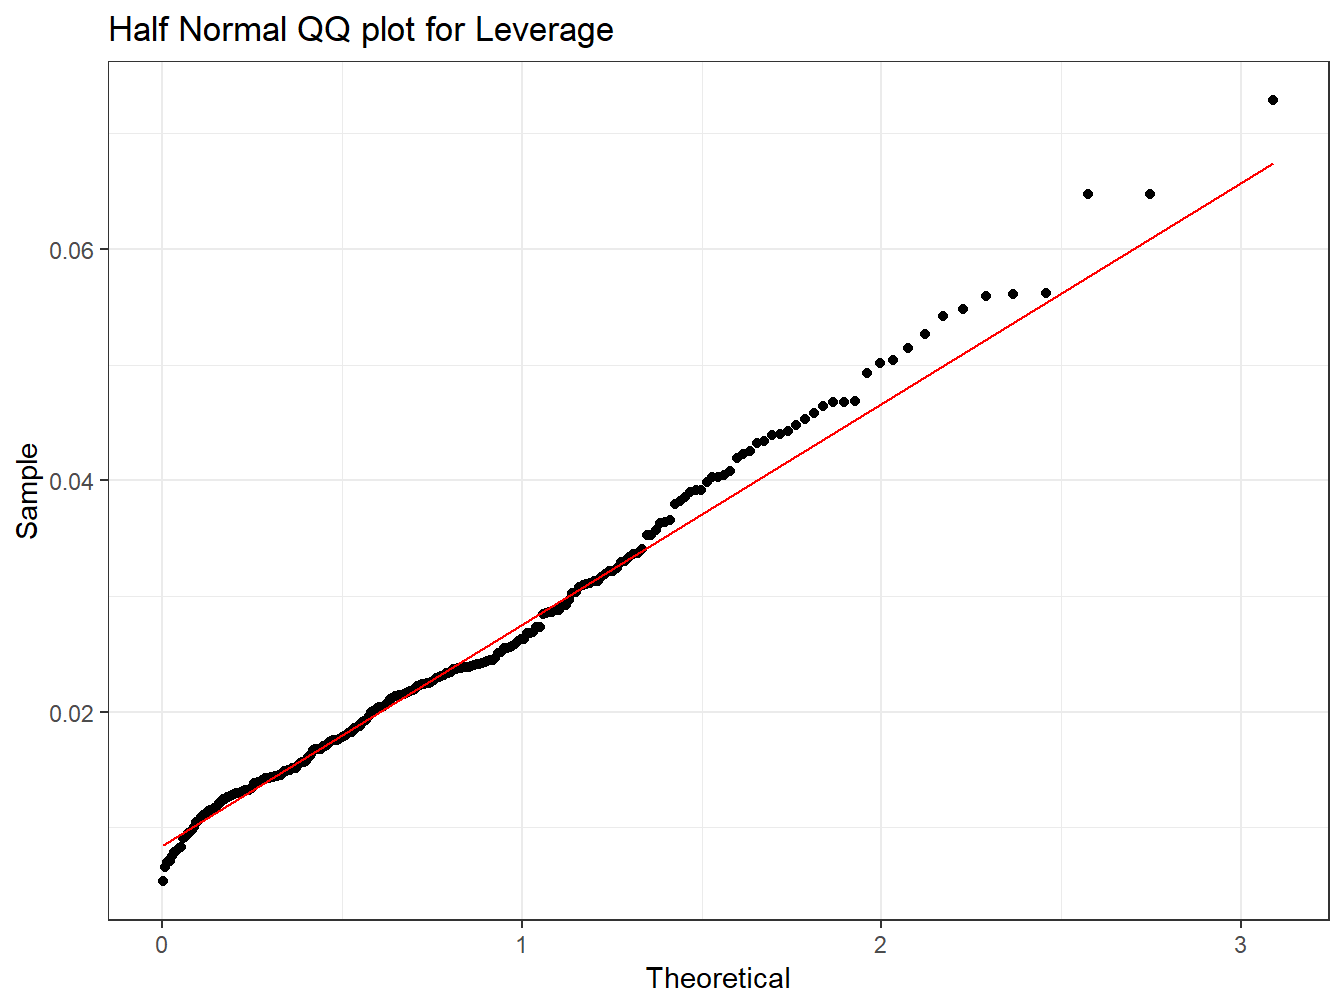
\includegraphics[width=0.8\linewidth]{final_exam_2_files/figure-latex/leverage-q2-1} 

}

\caption{Searching for Outliers with Large Influence}\label{fig:leverage-q2}
\end{figure}

However in Figure \ref{fig:cooks-q2} we can see that we have one very very large outlier. This value does not appear to be from the same model as the rest of the data.

\begin{figure}

{\centering 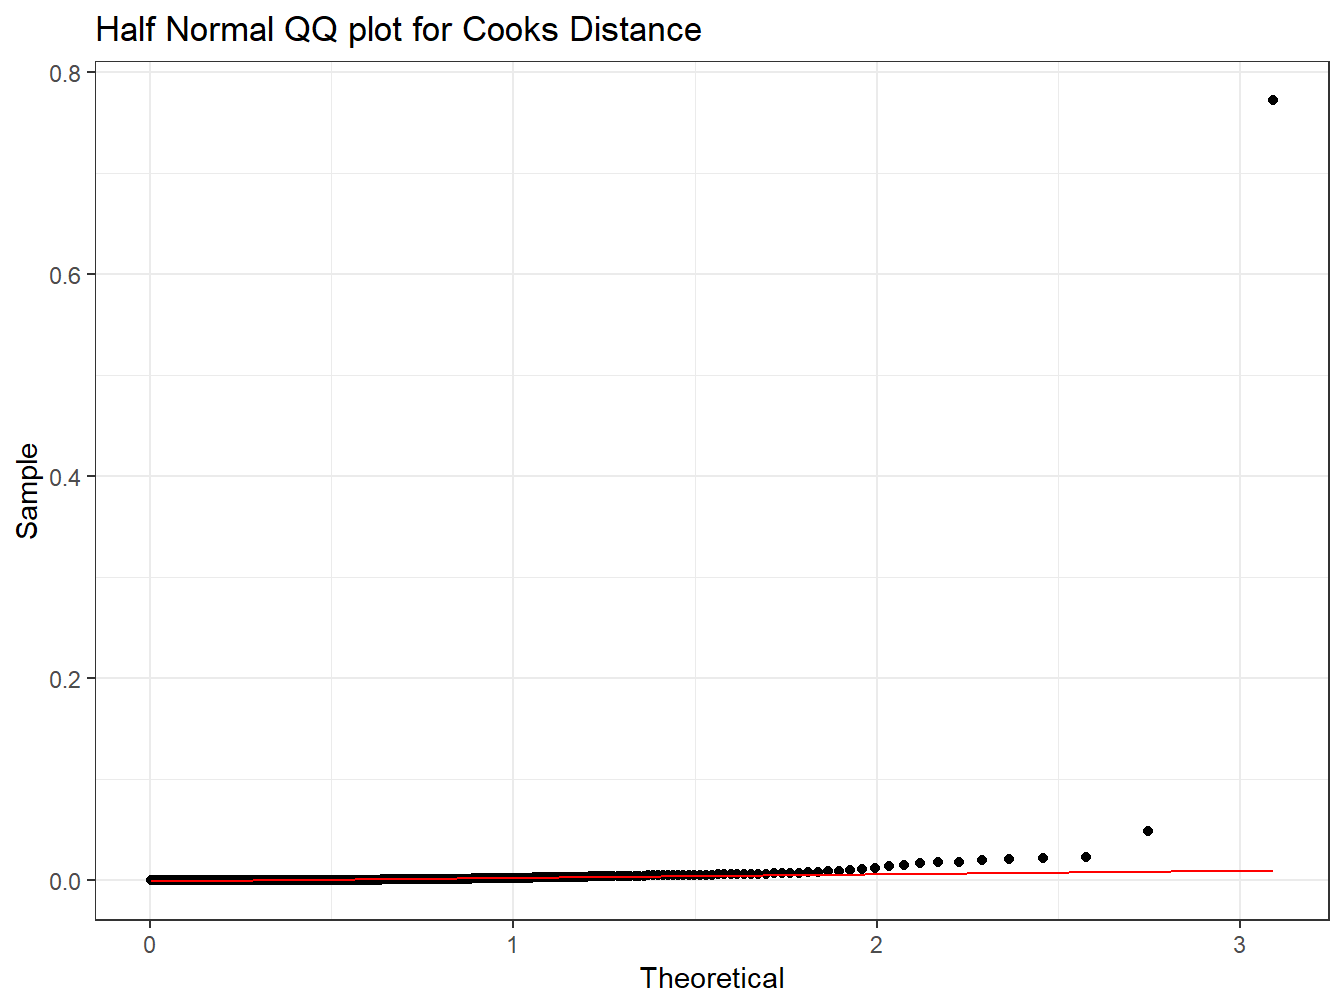
\includegraphics[width=0.8\linewidth]{final_exam_2_files/figure-latex/cooks-q2-1} 

}

\caption{Searching for Unlikely Observations}\label{fig:cooks-q2}
\end{figure}

We can see this clearly when we plot our fitted values vs the response in Figure \ref{fig:fit-v-response}.

\begin{figure}

{\centering 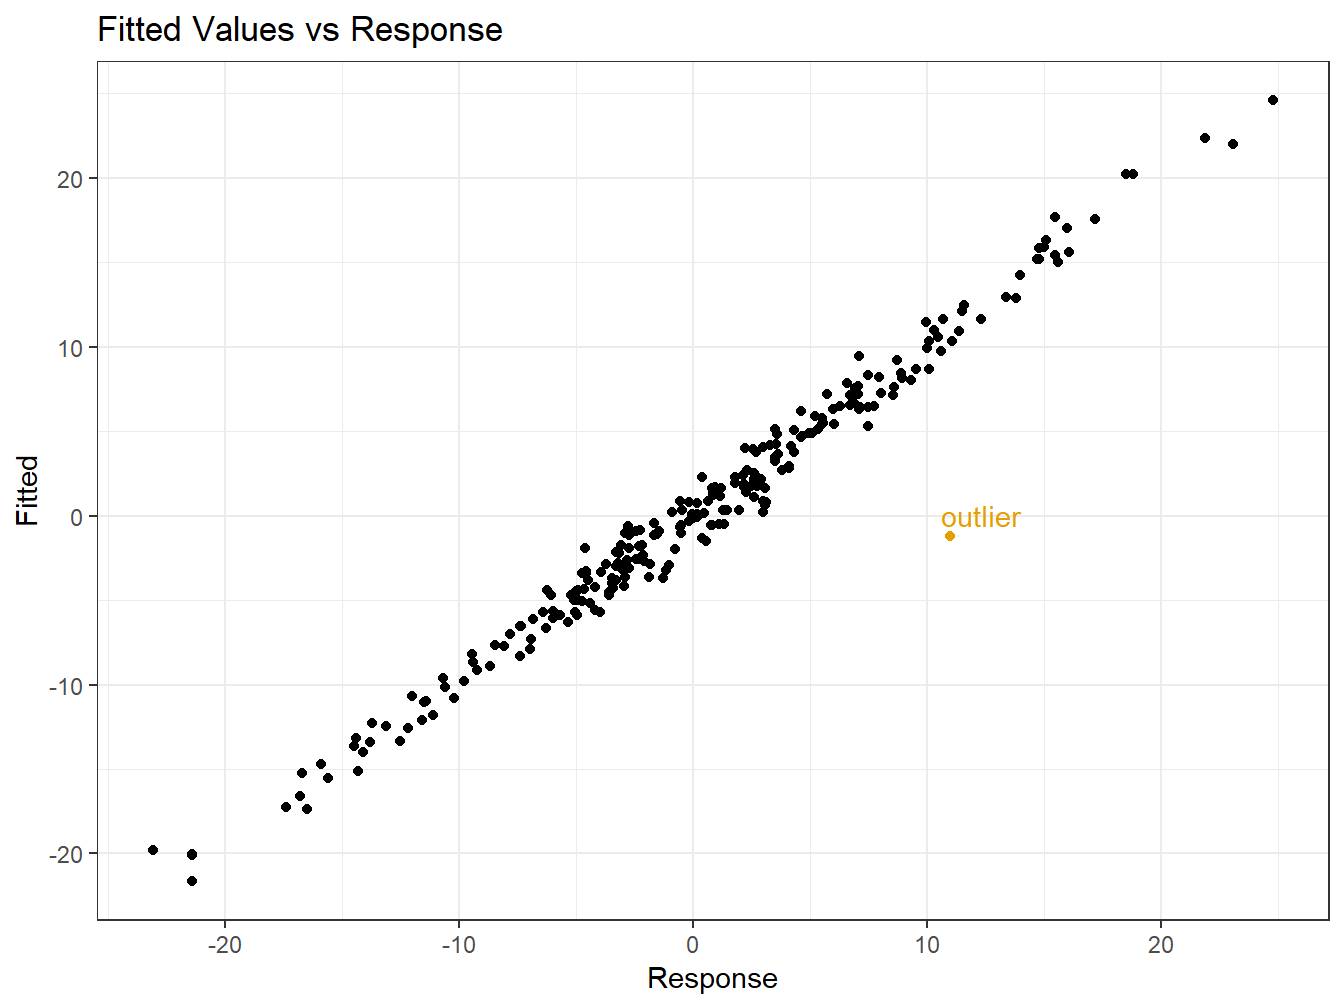
\includegraphics[width=0.8\linewidth]{final_exam_2_files/figure-latex/fit-v-response-1} 

}

\caption{Fitted Values vs Response with one big outlier}\label{fig:fit-v-response}
\end{figure}

If this was a real world situation I would investigate further about the data collection process and circumstances that led to this measurement. I would check to see if there was perhaps a data entry error or wheteher this is a realistic outcome.

Since I do not have that capacity here, I have decided to run a simulation to see how likely it was to see a residual of this size. For 10\^{}\{5\} simulations, I generated 250 random values from a normal distribution with mean 0 and a standard deviation of \(\hat{\sigma}\) (1.29). Out of those 10\^{}\{5\} simulations, there were 0 which had a value as or more extreme as the residual value we see for our big outlier.

As a result I will remove the point as it does not appear to be from the same model as the rest of the data. In the real world I would make a note that I have removed this point and watch to see if we see anything similar pop up again.

I will refit the model with this point removed before continuing on with any of the other assumption checking. We can see in table \ref{tab:coefs-no-outlier} that the new beta estimates have not changed much. This was to be expected becasue the outlier did not have a large leverage value. The updated estimate of \(\hat{\sigma}\) is 1.01.

\begin{table}

\caption{\label{tab:coefs-no-outlier}OLS regression coefficients with outlier removed}
\centering
\begin{tabular}[t]{lr}
\toprule
Term & Estimate\\
\midrule
Intercept & -0.02\\
Regressor 1 & 0.96\\
Regressor 2 & 1.87\\
Regressor 3 & -3.01\\
Regressor 4 & -4.06\\
Regressor 5 & -4.88\\
\bottomrule
\end{tabular}
\end{table}

We can now compare the half normal qq plot for cooks distance for the model with the outlier and without the outlier. The Figure \ref{fig:cooks-q2-2} shows the plot with the outlier and Figure \ref{fig:cooks-no-outlier-q2} shows the plot with the outlier removed.

\begin{figure}

{\centering 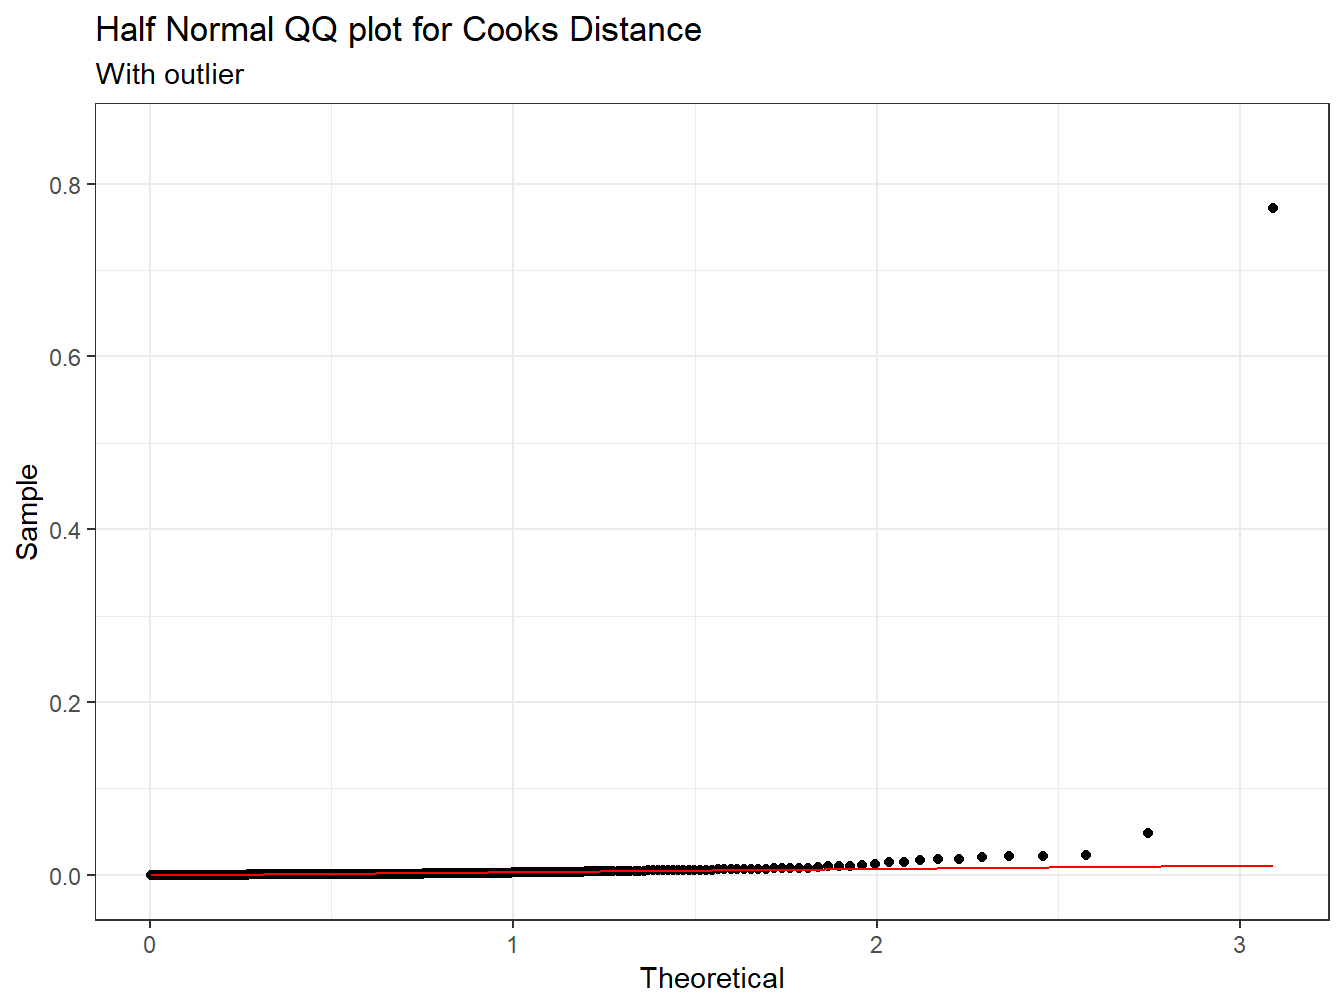
\includegraphics[width=0.8\linewidth]{final_exam_2_files/figure-latex/cooks-q2-2-1} 

}

\caption{Cooks Distance Before}\label{fig:cooks-q2-2}
\end{figure}

As they are set to the same scale we can see clearly that the diagnostic has improved after the outlier is removed.

\begin{figure}

{\centering 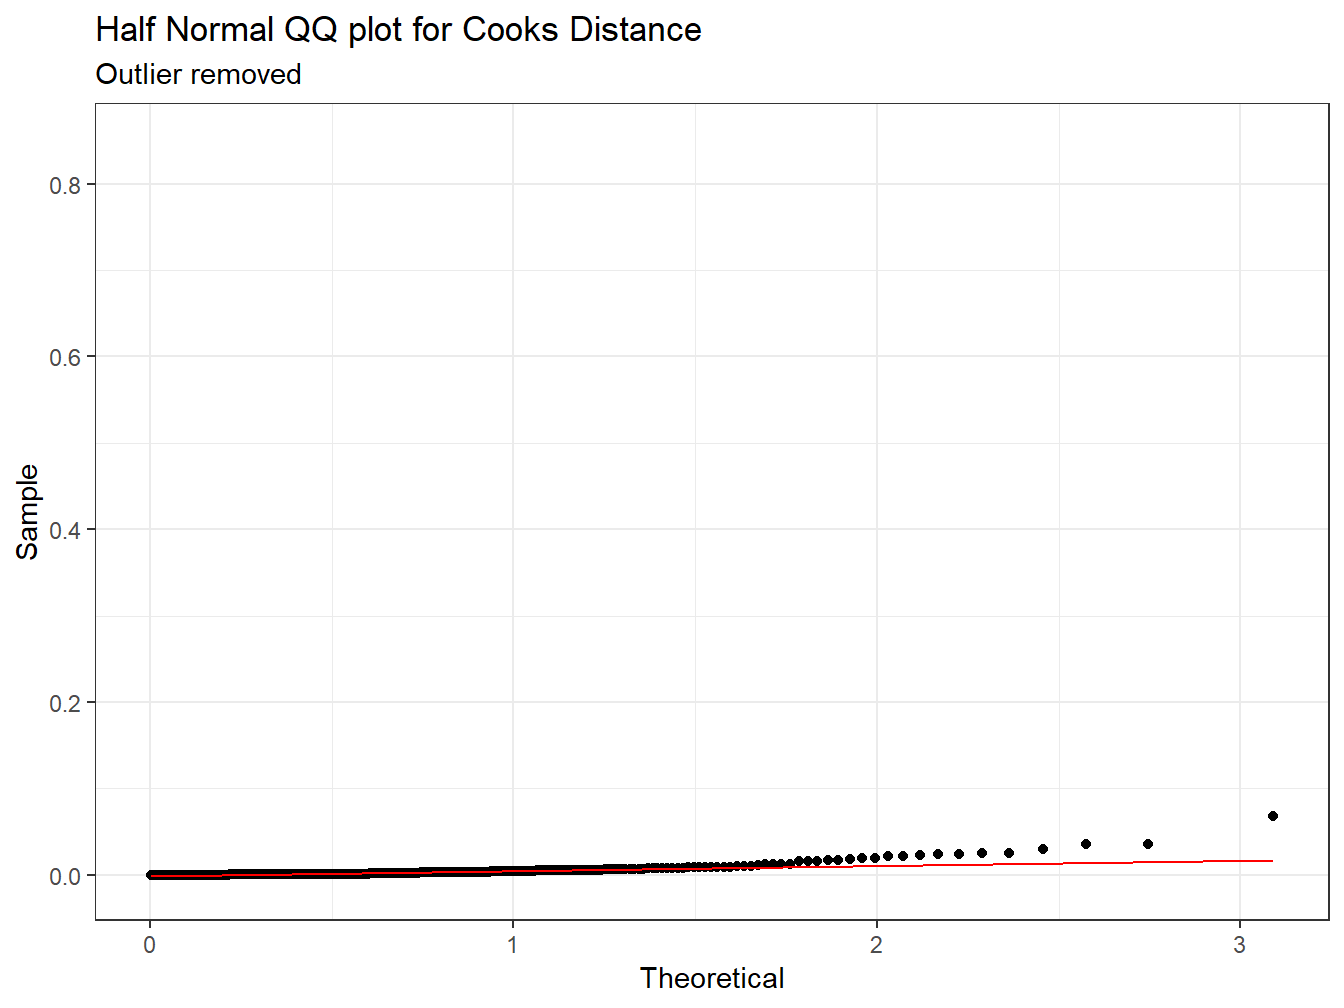
\includegraphics[width=0.8\linewidth]{final_exam_2_files/figure-latex/cooks-no-outlier-q2-1} 

}

\caption{Cooks Distance After}\label{fig:cooks-no-outlier-q2}
\end{figure}

Finally, I plot the half normal qq plot of the leverage after the outlier has been removed in Figure \ref{fig:lev-after} to show that we have not introduced any concerns by removing the observation.

\begin{figure}

{\centering 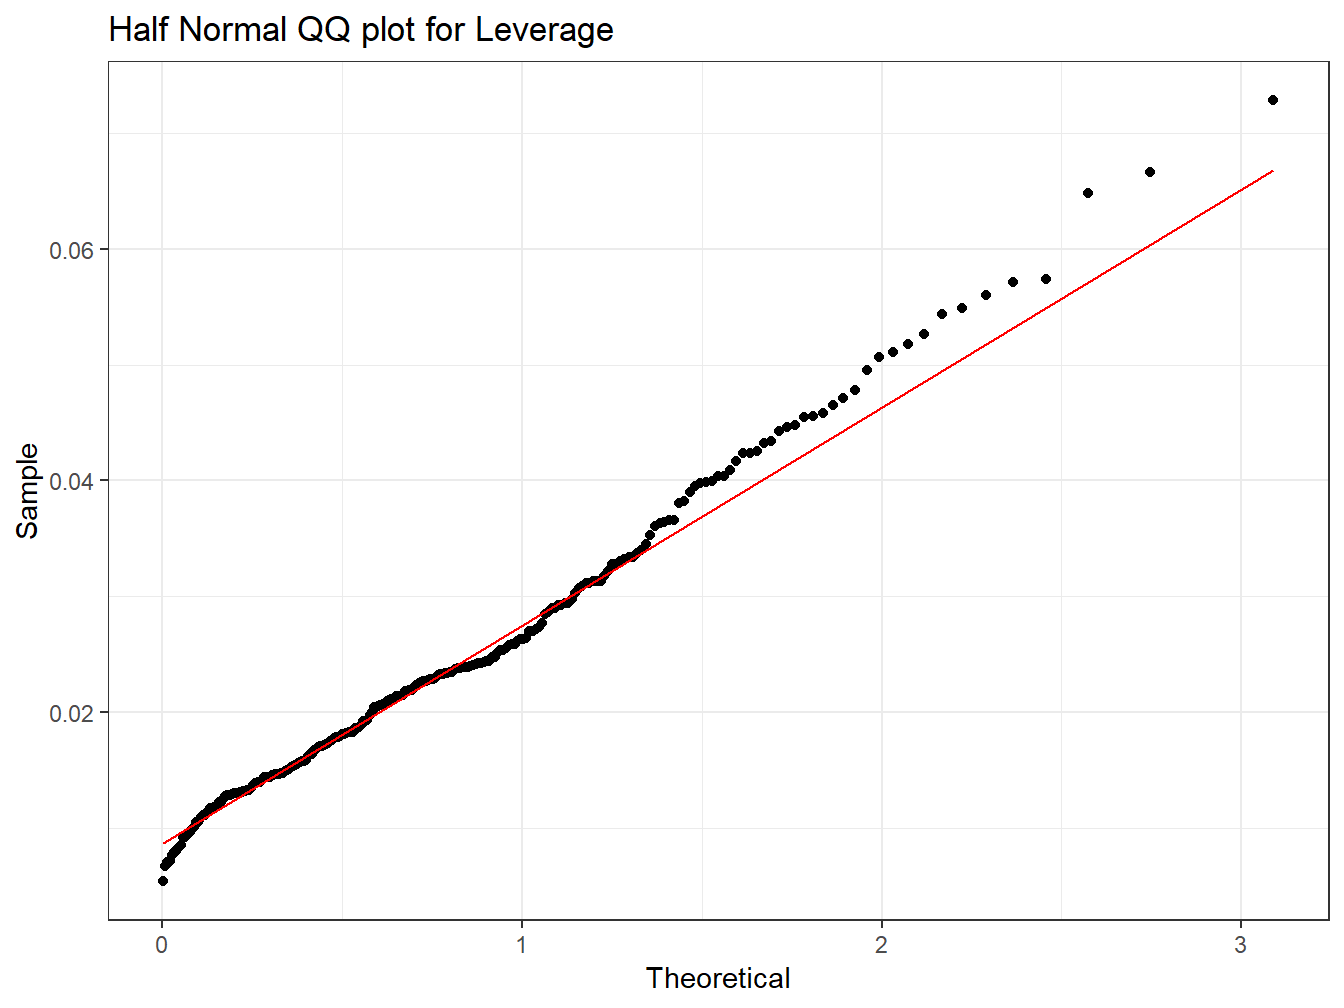
\includegraphics[width=0.8\linewidth]{final_exam_2_files/figure-latex/lev-after-1} 

}

\caption{Leverage After Outlier Removed}\label{fig:lev-after}
\end{figure}

We can now continue on with the rest of the model assumption checks.

\hypertarget{errors}{%
\subsection{Errors}\label{errors}}

I will now check to see if the residuals have equal variance, are normally distributed and are independent. To check for equal variance in the reisduals I plot the residuals against the fitted values in Figure \ref{fig:resid-fit-q2}. Using ``Loughins Thumb Test'', I do not see anything that would indicate that the constant variance assumption is violated.

\begin{figure}

{\centering 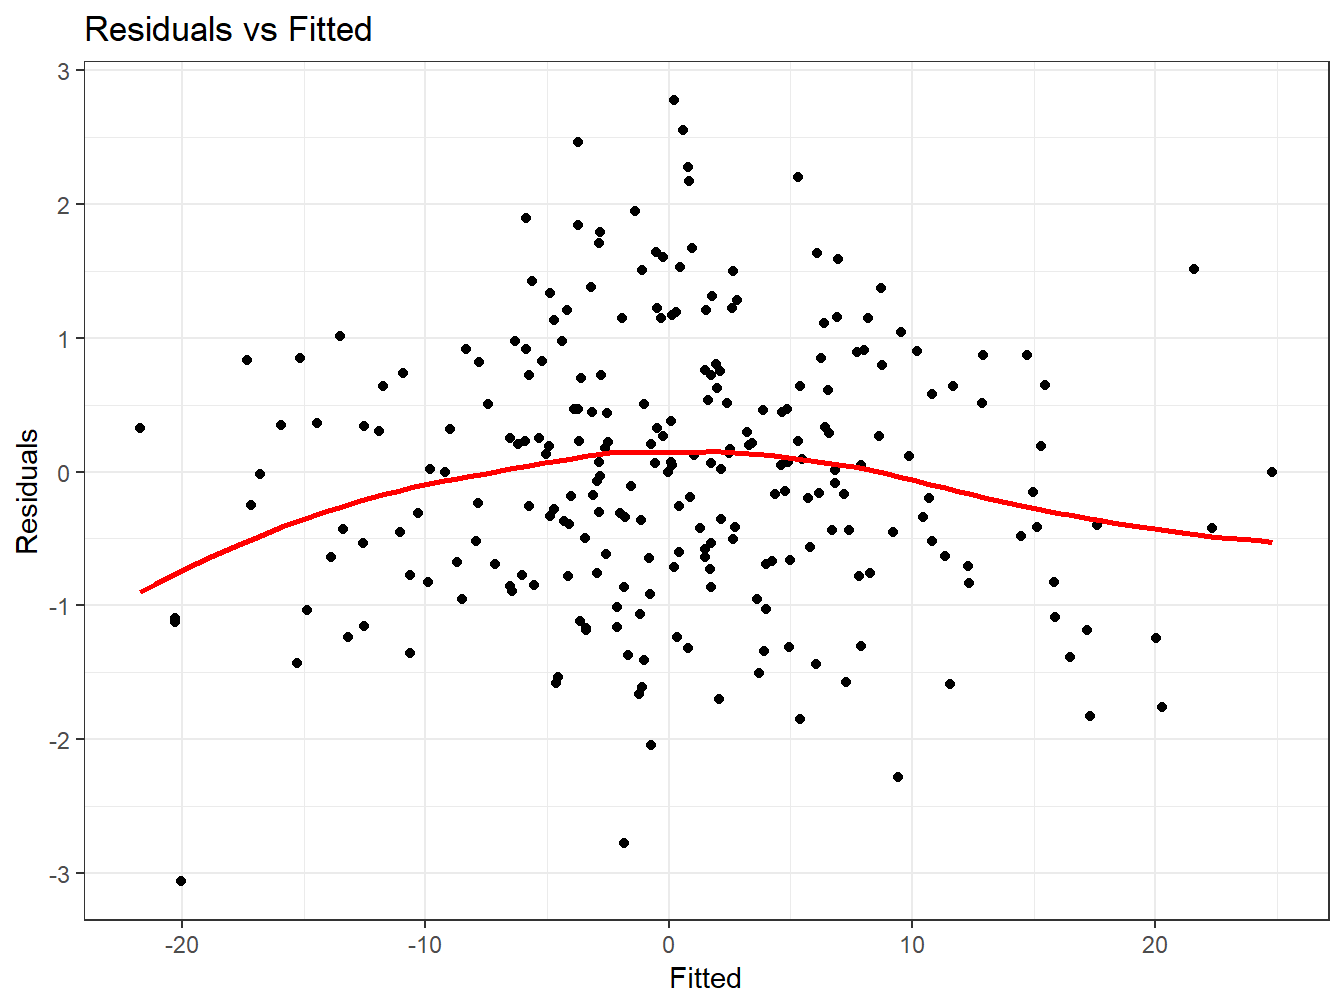
\includegraphics[width=0.8\linewidth]{final_exam_2_files/figure-latex/resid-fit-q2-1} 

}

\caption{Checking for constant variance}\label{fig:resid-fit-q2}
\end{figure}

Next I plotted a normal qq plot for the residuals to check to see if the data looks normally distributed. In Figure \ref{fig:qq-q2}, I do not see anything that would lead me to believe that the residuals are not normal.

\begin{figure}

{\centering 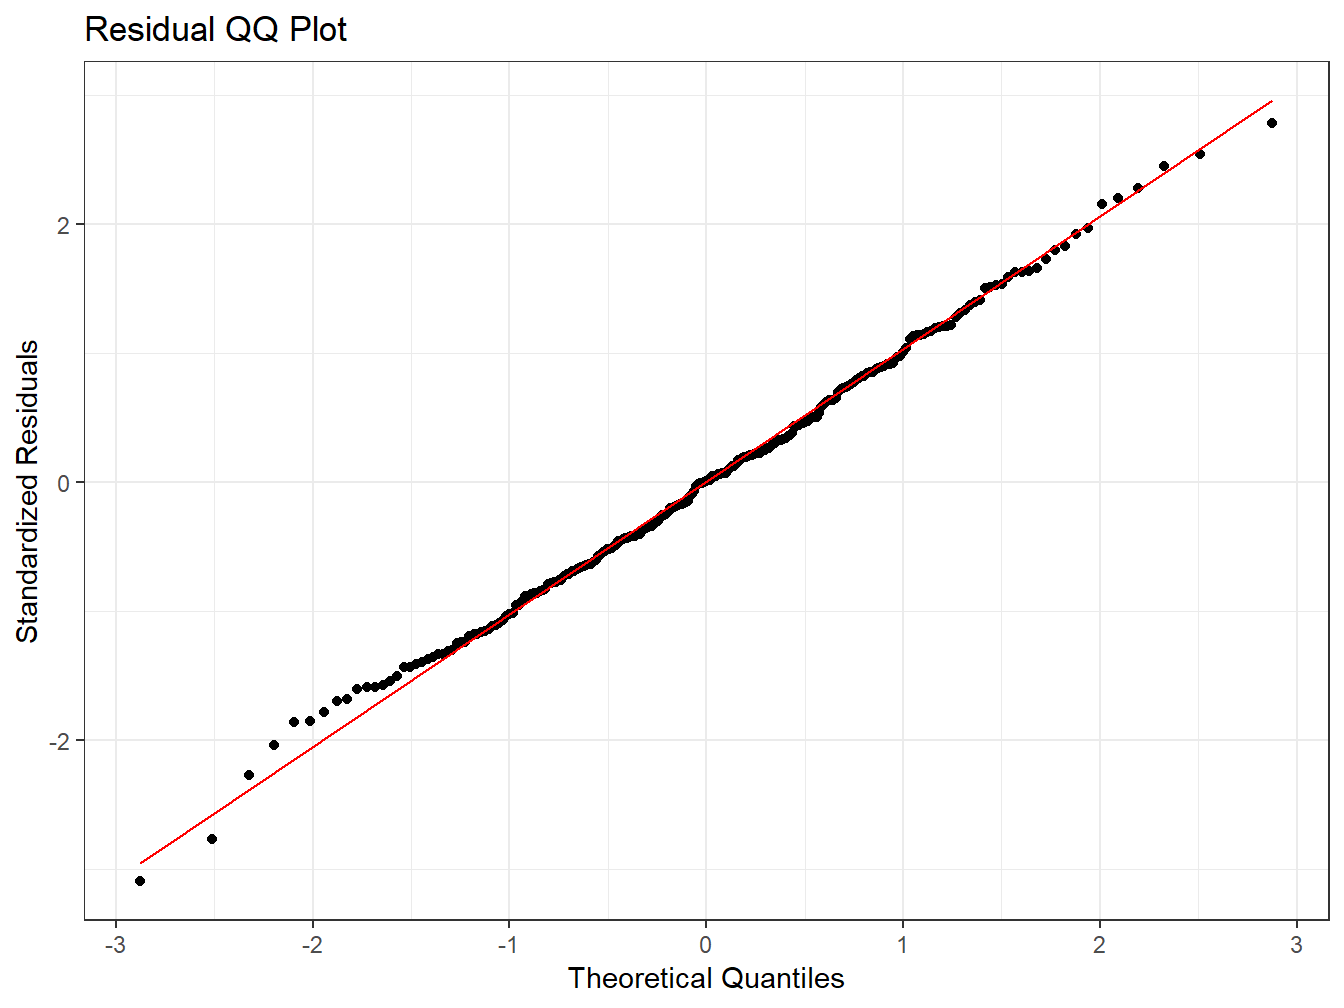
\includegraphics[width=0.8\linewidth]{final_exam_2_files/figure-latex/qq-q2-1} 

}

\caption{Checking for normality}\label{fig:qq-q2}
\end{figure}

Finally, I checked to see if I could find a reason why the residuals would not be independent. Since there is no practical interpretations for the data the best I could do was to plot the residuals by row number. In Figure \ref{fig:resid-order-q2}, it looks like the residuals are independent of the order in which the data was collected. Since there were no signs of autocorrelation I did not feel the need to include a Durbin Watson test.

\begin{figure}

{\centering 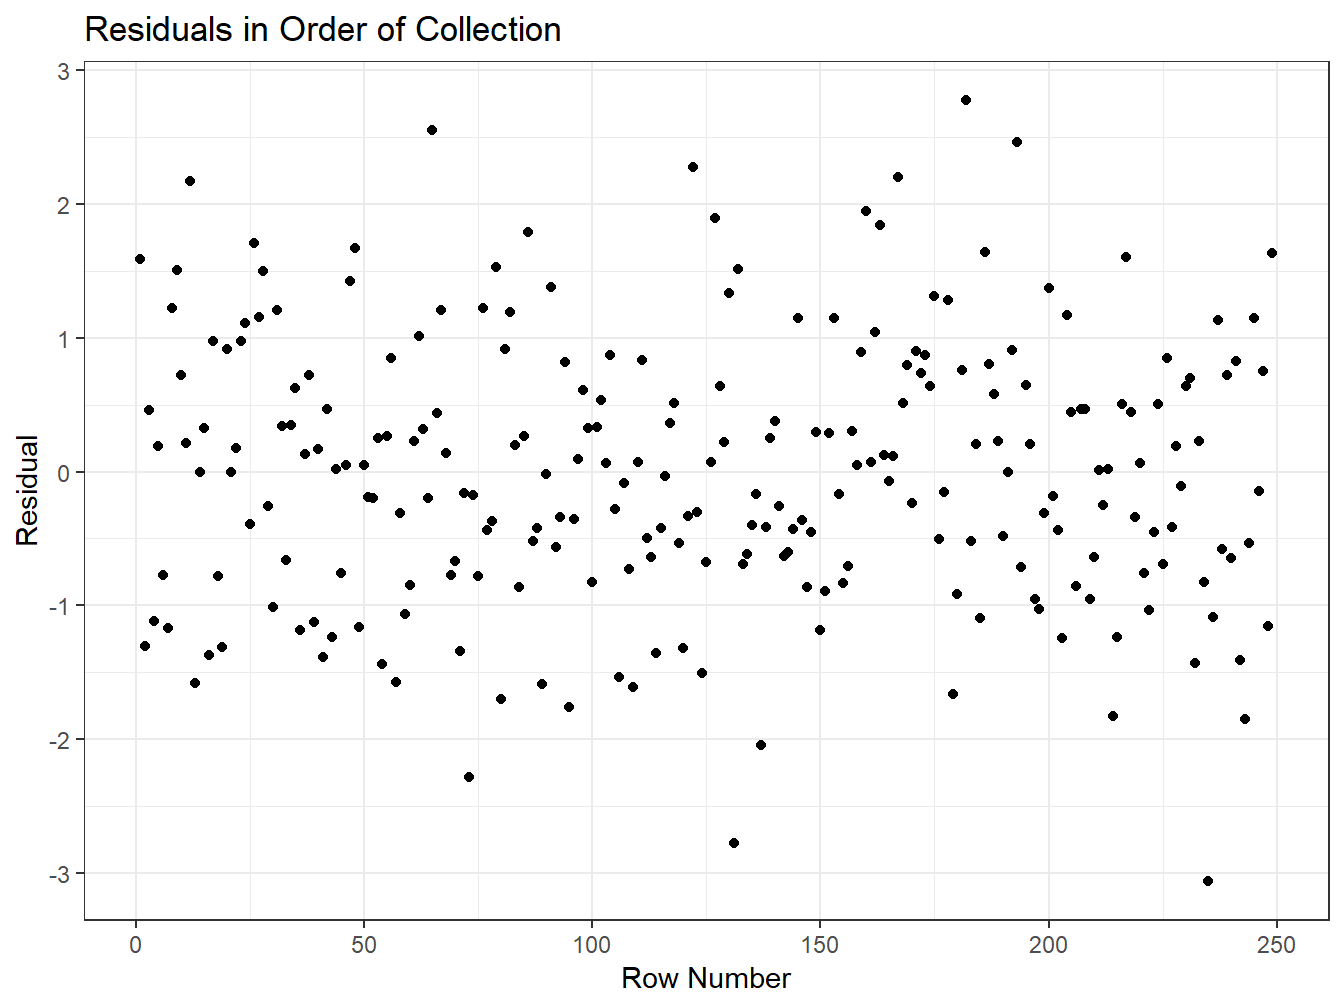
\includegraphics[width=0.8\linewidth]{final_exam_2_files/figure-latex/resid-order-q2-1} 

}

\caption{Checking for Independence of Order of Collection}\label{fig:resid-order-q2}
\end{figure}

\hypertarget{verify-model-choice}{%
\subsection{Verify Model Choice}\label{verify-model-choice}}

While it is not a perfect way to check the validity of the linear relationship we have assumed on the data because for any fixed value of a variable the other variables are changing, in Figure \ref{fig:pairs-q2} we can see that all of the regressors look like they have a linear relationship with the response. There is an argument to be made that Regressor 1 and 2 are unhelpful in explaing the reponse but again we are not sure how they change with respect to the other regressors.

\begin{figure}

{\centering 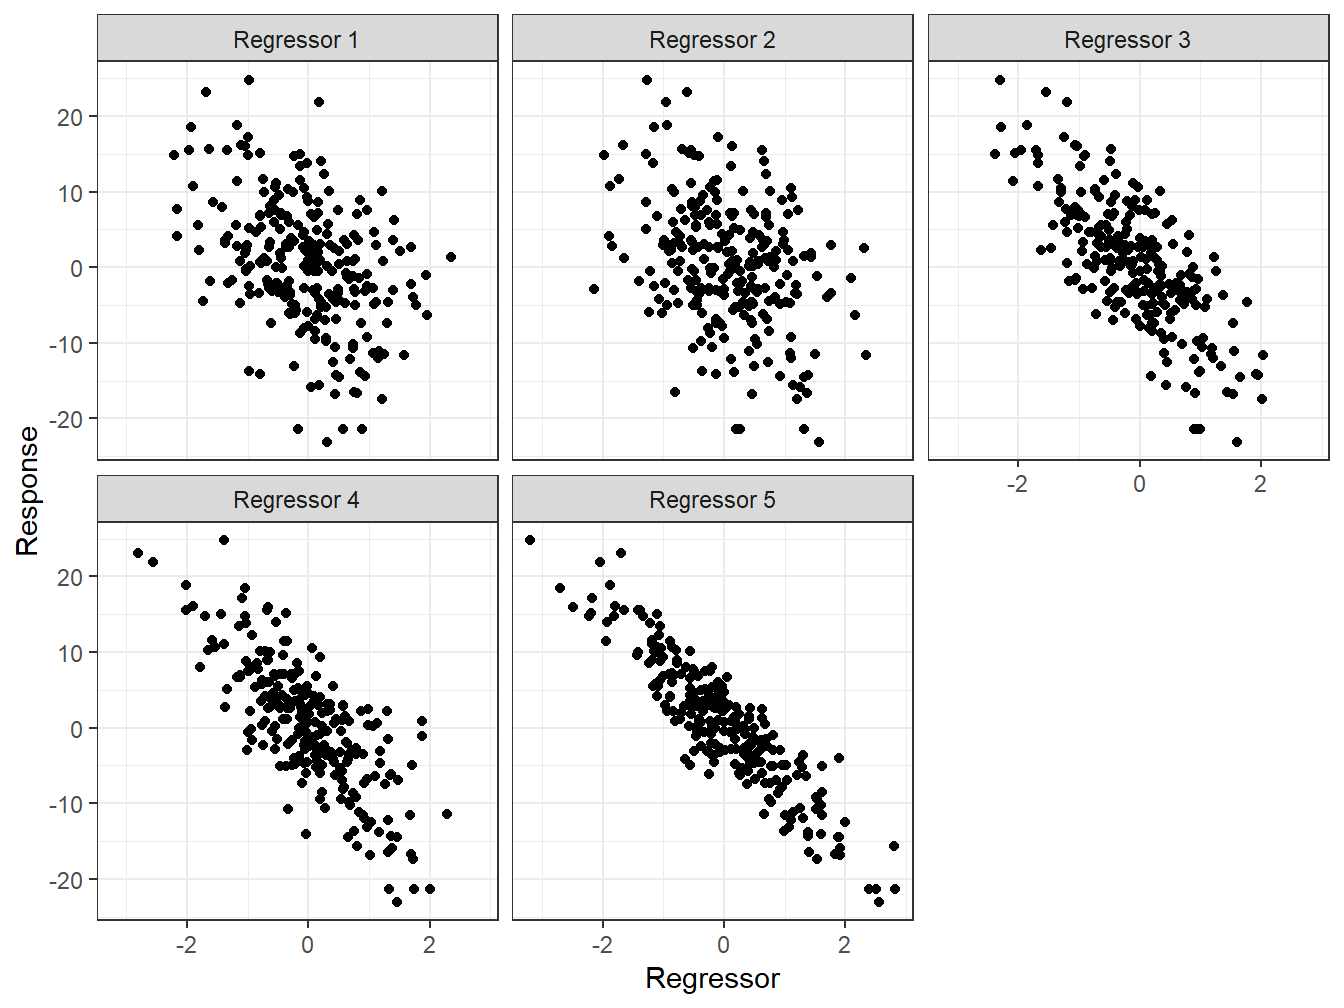
\includegraphics[width=0.8\linewidth]{final_exam_2_files/figure-latex/pairs-q2-1} 

}

\caption{Checking for linear relationships}\label{fig:pairs-q2}
\end{figure}

With that we have checked all the model assumptions. The only change we made was removing the large outlier from the dataset.

\hypertarget{part-d-1}{%
\section{Part D}\label{part-d-1}}

In Table \ref{tab:conf-ints-q2} there are the 95\% confidence intervals for the model coefficients.

\begin{table}

\caption{\label{tab:conf-ints-q2}95 percent Confidence Intervals for model coefficients}
\centering
\begin{tabular}[t]{lrrr}
\toprule
Term & Estimate & Conf Low & Conf High\\
\midrule
Intercept & -0.02 & -0.15 & 0.11\\
Regressor 1 & 0.96 & 0.77 & 1.15\\
Regressor 2 & 1.87 & 1.68 & 2.07\\
Regressor 3 & -3.01 & -3.22 & -2.81\\
Regressor 4 & -4.06 & -4.25 & -3.86\\
Regressor 5 & -4.88 & -5.06 & -4.70\\
\bottomrule
\end{tabular}
\end{table}

\hypertarget{part-e}{%
\section{Part E}\label{part-e}}

In Figure \ref{fig:joint-conf-q2} I plotted a joint 95\% confidence region for \(\beta_1\) and \(\beta_2\). This region can be used to test the null hypothesis

\begin{align}
  \beta_1 &= \beta_2 = 0
\end{align}

Against the alternative hypothesis that

\begin{align}
  \beta_1 \neq 0\ &|\ \beta_2 \neq 0
\end{align}

Since the region does not overlap with the original we can reject the null hypothesis in favour of the alternative hypothesis that both coefficients are not equal to 0 at the \(\alpha = 0.05\) level.

\begin{figure}

{\centering 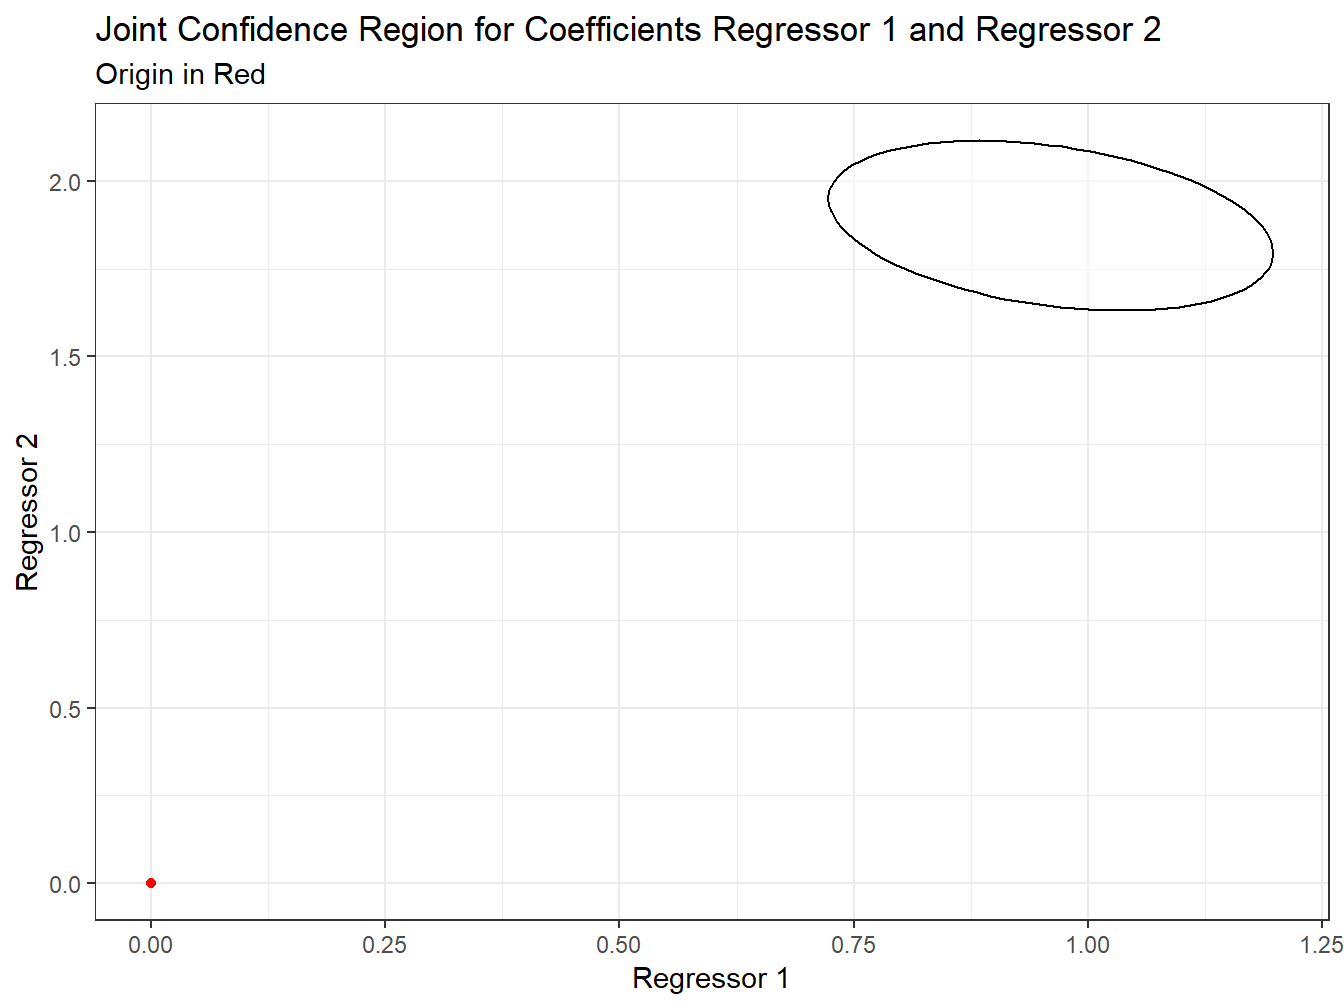
\includegraphics[width=0.8\linewidth]{final_exam_2_files/figure-latex/joint-conf-q2-1} 

}

\caption{Joint 95 percent Confidence Interval for Regressor 1 and Regressor 2}\label{fig:joint-conf-q2}
\end{figure}

\hypertarget{part-f}{%
\section{Part F}\label{part-f}}

Using the data with the outlier removed I fit ridge regression models for \(\lambda\) values between 0 and 50. As a result I have plotted in Figure \ref{fig:ridge-coef-q2} the coefficients of the various regressors at each \(\lambda\) value. Since the best lambda, the one with the smallesti cross validation mean squared error, is 0, the best model is actually the one without penalization. This is telling us that the model we should use is the one with the OLS coefficient estimates. These coefficient estimates are displayed in Table \ref{tab:coefs-no-outlier}.

\begin{figure}

{\centering 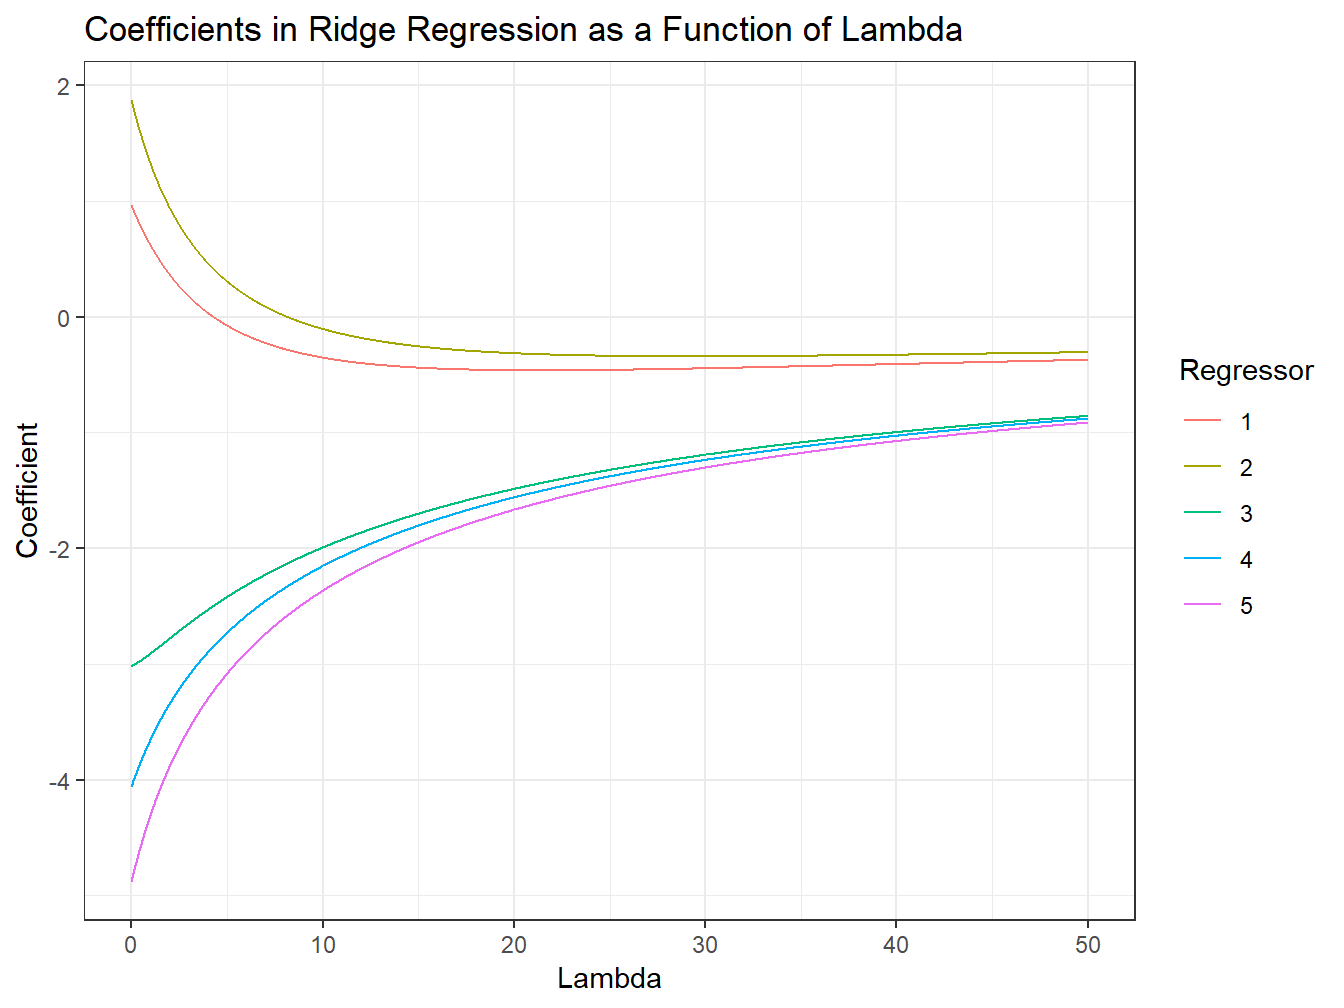
\includegraphics[width=0.8\linewidth]{final_exam_2_files/figure-latex/ridge-coef-q2-1} 

}

\caption{Ridge Regression Coefficients as Lambda Varies}\label{fig:ridge-coef-q2}
\end{figure}

\hypertarget{part-g}{%
\section{Part G}\label{part-g}}

I performed forward selection using AIC as my evaluation metric and an implementation provided by the MASS package. Again, the full model is suggested as the best one. The coefficient estimates are in Table \ref{tab:coefs-no-outlier}.

\hypertarget{part-h}{%
\section{Part H}\label{part-h}}

Given that both model selection techniques returned the OLS model, if I knew that each coefficient was originally an integer I would simply round the coefficients to the nearest integer to get the values in Table \ref{tab:coefs-rounded-q2}

\begin{table}

\caption{\label{tab:coefs-rounded-q2}OLS regression coefficients with outlier removed rounded to nearest integer}
\centering
\begin{tabular}[t]{lr}
\toprule
Term & Estimate\\
\midrule
Intercept & 0\\
Regressor 1 & 1\\
Regressor 2 & 2\\
Regressor 3 & -3\\
Regressor 4 & -4\\
Regressor 5 & -5\\
\bottomrule
\end{tabular}
\end{table}

\hypertarget{question-3}{%
\chapter{Question 3}\label{question-3}}

\hypertarget{part-a-2}{%
\section{Part A}\label{part-a-2}}

I simulated 1000 different responses from the true model and estimated the model parameters using a OLS regression. The mean of the estimated model parameters over all the simulations are displayed in Table \ref{tab:lm-mean-coefs-q3}. They are quite close to the true value of the model parameters (as a reminder \(\beta_0 = 1,\ \beta_1 = 2,\ \beta_2 = 3\)). Additionally, in Table \ref{tab:theory-vcov-q3} we have the theoretical covariance matrix of the model parameters so that we can compare the mean estimated covariance matrix of the estimated model parameters from the 1000 simulations that is displayed in table \ref{tab:lm-est-vcov-q3}

\begin{table}

\caption{\label{tab:lm-mean-coefs-q3}Mean of model coefficients from OLS model over 1000 simulations}
\centering
\begin{tabular}[t]{lr}
\toprule
Term & Mean\\
\midrule
Intercept & 0.987\\
Regressor 1 & 2.000\\
Regressor 2 & 3.020\\
\bottomrule
\end{tabular}
\end{table}

\begin{table}

\caption{\label{tab:theory-vcov-q3}Theoretical covariance matrix of the model parameters}
\centering
\begin{tabular}[t]{lrrr}
\toprule
Term & Intercept & Regressor 1 & Regressor 2\\
\midrule
Intercept & 0.032600 & 0.000661 & -0.052200\\
Regressor 1 & 0.000661 & 0.005310 & -0.000863\\
Regressor 2 & -0.052200 & -0.000863 & 0.103000\\
\bottomrule
\end{tabular}
\end{table}

\begin{table}

\caption{\label{tab:lm-est-vcov-q3}Mean of the estimated covariance matrix of the OLS model parameters over 1000 simulations}
\centering
\begin{tabular}[t]{lrrr}
\toprule
Term & Intercept & Regressor 1 & Regressor 2\\
\midrule
Intercept & 0.032400 & 0.000657 & -0.051900\\
Regressor 1 & 0.000657 & 0.005270 & -0.000857\\
Regressor 2 & -0.051900 & -0.000857 & 0.103000\\
\bottomrule
\end{tabular}
\end{table}

\hypertarget{part-b-2}{%
\section{Part B}\label{part-b-2}}

For the same 1000 simulated data sets I took a Bayesian approach to estimate the model parameters.

I used the following priors,

\begin{align}
  \beta &\sim N \bigg( 
  \begin{bmatrix}
  0\\
  0\\
  0\\
  \end{bmatrix},
  5 \begin{bmatrix}
  1 & 0 & 0\\
  0 & 1 & 0\\
  0 & 0 & 1\\
  \end{bmatrix} \bigg)\\
  \sigma^2 &\sim IG(2, 0.5)
\end{align}

The marginal posterior distribution for the vector \(\beta\) is a multivariate t distribution which has mean \(\mu_\text{new}\) where

\begin{align}
  \mu_\text{new} &= (\Sigma^{-1} + X^T X)^{-1} (\Sigma^{-1} \mu + X^T y)
\end{align}

and the marginal posterior distribution for \(\sigma^2\) is a Inverse Gamma distribution with parameters \(a_\text{new}\) and \(b_\text{new}\) which are defined to be,

\begin{align}
  a_\text{new} &= a + n/2\\
  b_\text{new} &= b + \frac{1}{2}[\mu^T \Sigma^{-1} \mu + y^T y - \mu_\text{new}^T \Sigma_\text{new}^{-1} \mu_\text{new}]
\end{align}

and

\begin{align*}
  \Sigma_\text{new} &= (\Sigma^{-1} + X^T X)^{-1}
\end{align*}

the mean of an Inverse Gamma distribution is \(\frac{b}{a - 1}\)

The mean of the estimated model parameters over all the simulations using the posterior means are displayed in Table \ref{tab:bayes-b-mean-coefs-q3}. They are a little farther away from the true parameters than the OLS mean estimates. Regressor 1 is close to the true value.

We can compare the mean estimated covariance matrix of the estimated model parameters from the 1000 simulations that is displayed in table \ref{tab:bayes-b-est-vcov-q3} to the theoretical covariance matrix of the model parameters that I have reprinted in table \ref{tab:theory-vcov-b-q3} for convenience. We are much farther away from the theoretical covariance matrix then in the linear model case.

\begin{table}

\caption{\label{tab:bayes-b-mean-coefs-q3}Mean of model coefficients from Bayesian model in part b over 1000 simulations}
\centering
\begin{tabular}[t]{lr}
\toprule
Regressor & Mean\\
\midrule
Intercept & 1.30\\
Regressor 1 & 1.96\\
Regressor 2 & 2.33\\
\bottomrule
\end{tabular}
\end{table}

\begin{table}

\caption{\label{tab:bayes-b-est-vcov-q3}Estimated covariance matrix of the model parameters for bayesian model in part b}
\centering
\begin{tabular}[t]{lrrr}
\toprule
Term & Intercept & Regressor 1 & Regressor 2\\
\midrule
Intercept & 0.07000 & 0.00142 & -0.11200\\
Regressor 1 & 0.00142 & 0.01140 & -0.00185\\
Regressor 2 & -0.11200 & -0.00185 & 0.22200\\
\bottomrule
\end{tabular}
\end{table}

\begin{table}

\caption{\label{tab:theory-vcov-b-q3}Theoretical covariance matrix of the model parameters}
\centering
\begin{tabular}[t]{lrrr}
\toprule
Term & Intercept & Regressor 1 & Regressor 2\\
\midrule
Intercept & 0.032600 & 0.000661 & -0.052200\\
Regressor 1 & 0.000661 & 0.005310 & -0.000863\\
Regressor 2 & -0.052200 & -0.000863 & 0.103000\\
\bottomrule
\end{tabular}
\end{table}

\hypertarget{part-c-2}{%
\section{Part C}\label{part-c-2}}

I changed the priors according to part c to be,

\begin{align}
  \beta &\sim N \bigg( 
  \begin{bmatrix}
  1\\
  1\\
  1\\
  \end{bmatrix},
  1 \begin{bmatrix}
  1 & 0 & 0\\
  0 & 2 & 0\\
  0 & 0 & 3\\
  \end{bmatrix} \bigg)\\
  \sigma^2 &\sim IG(2, 0.5)
\end{align}

I then used the same update rule to find the means of the posterior distributions for the vector \(\beta\) and for \(\sigma^2\).

The mean of the estimated model parameters over all the simulations using the posterior means are displayed in Table \ref{tab:bayes-c-mean-coefs-q3}. They are a closer to the true values than the first prior was (which brought the values closer to 0) but still a little farther away from the true parameters than the OLS mean estimates.

We are closer in table \ref{tab:bayes-c-est-vcov-q3} to the theoretical covariance matrix of the model parameters in table \ref{tab:theory-vcov-c-q3} than the first bayesian approach was.

\begin{table}

\caption{\label{tab:bayes-c-mean-coefs-q3}Mean of model coefficients from Bayesian model in part c over 1000 simulations}
\centering
\begin{tabular}[t]{lr}
\toprule
Regressor & Mean\\
\midrule
Intercept & 1.10\\
Regressor 1 & 1.99\\
Regressor 2 & 2.80\\
\bottomrule
\end{tabular}
\end{table}

\begin{table}

\caption{\label{tab:bayes-c-est-vcov-q3}Estimated covariance matrix of the model parameters for bayesian model in part c}
\centering
\begin{tabular}[t]{lrrr}
\toprule
Term & Intercept & Regressor 1 & Regressor 2\\
\midrule
Intercept & 0.037100 & 0.000752 & -0.059400\\
Regressor 1 & 0.000752 & 0.006040 & -0.000981\\
Regressor 2 & -0.059400 & -0.000981 & 0.118000\\
\bottomrule
\end{tabular}
\end{table}

\begin{table}

\caption{\label{tab:theory-vcov-c-q3}Theoretical covariance matrix of the model parameters}
\centering
\begin{tabular}[t]{lrrr}
\toprule
Term & Intercept & Regressor 1 & Regressor 2\\
\midrule
Intercept & 0.032600 & 0.000661 & -0.052200\\
Regressor 1 & 0.000661 & 0.005310 & -0.000863\\
Regressor 2 & -0.052200 & -0.000863 & 0.103000\\
\bottomrule
\end{tabular}
\end{table}

\hypertarget{part-d-2}{%
\section{Part D}\label{part-d-2}}

Finally, in part d I used the following priors,

\begin{align}
  \beta &\sim N \bigg( 
  \begin{bmatrix}
  1\\
  1\\
  1\\
  \end{bmatrix},
  0.1 \begin{bmatrix}
  1 & 0 & 0\\
  0 & 1 & 0\\
  0 & 0 & 1\\
  \end{bmatrix} \bigg)\\
  \sigma^2 &\sim IG(2, 0.5)
\end{align}

The mean of the estimated model parameters over all the simulations using the posterior means are displayed in Table \ref{tab:bayes-d-mean-coefs-q3}. They are a little closer to the true parameters than the ones from part b but not by much. They are farther away from the true parameters than those in part c.

The estimated covariance matrix of the estimated model parameters in table \ref{tab:bayes-d-est-vcov-q3} are father away from the theoretical ones in table \ref{tab:theory-vcov-d-q3} than the matrix from part b but again not as close as the matrix in part c.

\begin{table}

\caption{\label{tab:bayes-d-mean-coefs-q3}Mean of model coefficients from Bayesian model in part d over 1000 simulations}
\centering
\begin{tabular}[t]{lr}
\toprule
Regressor & Mean\\
\midrule
Intercept & 1.26\\
Regressor 1 & 1.98\\
Regressor 2 & 2.47\\
\bottomrule
\end{tabular}
\end{table}

\begin{table}

\caption{\label{tab:bayes-d-est-vcov-q3}Estimated covariance matrix of the model parameters for bayesian model in part d}
\centering
\begin{tabular}[t]{lrrr}
\toprule
Term & Intercept & Regressor 1 & Regressor 2\\
\midrule
Intercept & 0.044200 & 0.000896 & -0.07080\\
Regressor 1 & 0.000896 & 0.007190 & -0.00117\\
Regressor 2 & -0.070800 & -0.001170 & 0.14000\\
\bottomrule
\end{tabular}
\end{table}

\begin{table}

\caption{\label{tab:theory-vcov-d-q3}Theoretical covariance matrix of the model parameters}
\centering
\begin{tabular}[t]{lrrr}
\toprule
Term & Intercept & Regressor 1 & Regressor 2\\
\midrule
Intercept & 0.032600 & 0.000661 & -0.052200\\
Regressor 1 & 0.000661 & 0.005310 & -0.000863\\
Regressor 2 & -0.052200 & -0.000863 & 0.103000\\
\bottomrule
\end{tabular}
\end{table}

\hypertarget{part-e-1}{%
\section{Part E}\label{part-e-1}}

Knowing the true parameter values, the Bayesian model in part c (with prior pulling \(\beta\) s to 1 and 1, 2 and 3 down the diagonal of the \(\Sigma\) matrix) was the most accurate over the 1000 simulations. We can see that the model in part b pulled the estimate for Regressor 2 too far towards 0. It is interesting to see that the estimate for the Intercept was actually an overestimate.

\hypertarget{part-f-1}{%
\section{Part F}\label{part-f-1}}

If I did not know the true parameter values and I was handed a dataset where I had no knowledge of the situation and no one to ilicit a prior belief from I think I would use the OLS frequentist approach. It is clear that in this case that the frequentist approach is better. However, I think if there was more information about the problem it would be better to incorporate it into the model and take a Bayesian approach.

\hypertarget{question-4}{%
\chapter{Question 4}\label{question-4}}

\hypertarget{part-a-3}{%
\section{Part A}\label{part-a-3}}

In Figure \ref{fig:exp-plot-q4} we can begin to explore the relationships of Density and Impurity with Absorbtion Rate. We can see that Impurity is Low that the Absorbtion Rate has a similar mean regardless of the density of the graphite. However, if the garphite impurity is high then there is fairly clear difference in absorbtion rate for high density and low density graphite.

\begin{figure}

{\centering 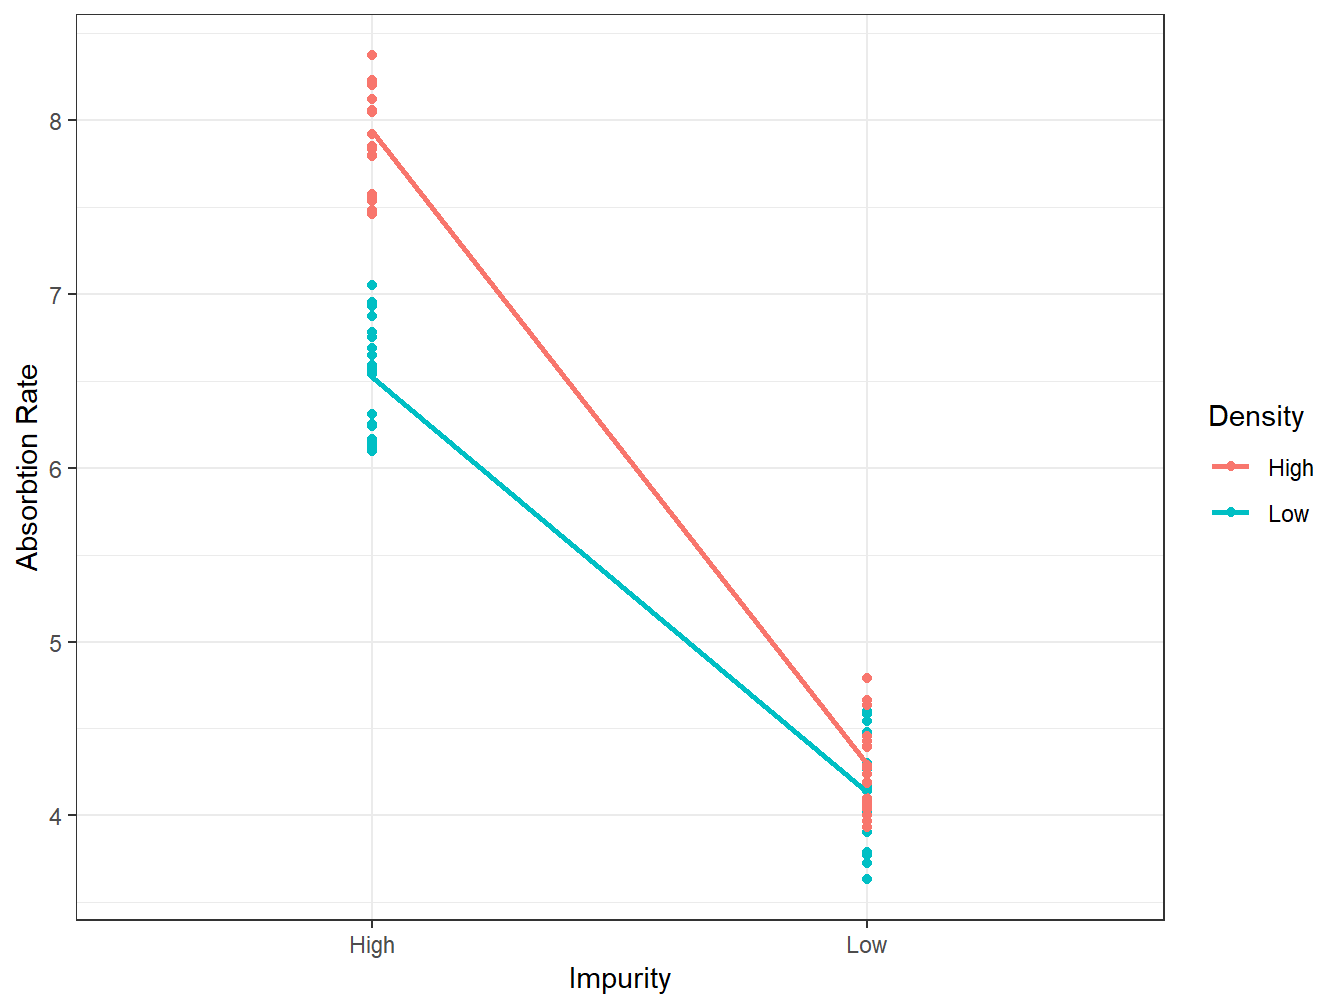
\includegraphics[width=0.8\linewidth]{final_exam_2_files/figure-latex/exp-plot-q4-1} 

}

\caption{Radioactive neutrons and graphite bricks}\label{fig:exp-plot-q4}
\end{figure}

\hypertarget{part-b-3}{%
\section{Part B}\label{part-b-3}}

A suitable model for this experiment would be

\begin{align}
  y &= \beta_0 + \beta_1 I(\text{Impurity = Low}) + \beta_2 I(\text{Density = Low}) + \beta_3 I(\text{Impurity = Low}) I(\text{Density = Low}) + \epsilon
\end{align}

This uses the High/High Impurity/Density combination the baseline Intercept and the other effects are deviations form this baseline. \(\epsilon \sim N(0, \sigma^2)\)

\hypertarget{part-c-3}{%
\section{Part C}\label{part-c-3}}

I tested for each \(\beta_i\) the null hypothesis that \(\beta_i = 0\) against the alternative hypothesis \(\beta_i \neq 0\). The test statistic reported is a t-statistic with 77 degrees of freedom. We will perform these tests each at a \(\alpha = 0.05\) level which does not adjust for the multiple comparisons that are being made. In Table \ref{tab:beta-test-q4} the model estimates and test results are displayed. All tests for the \(\beta_i\) have the null hypothesis that \(\beta_i = 0\) rejected. I will now test furthur to see which levels of combinations have different means.

\begin{table}

\caption{\label{tab:beta-test-q4}Beta estimates and test results}
\centering
\begin{tabular}[t]{lrrrr}
\toprule
Term & Estimate & Std Error & Statistic & P Value\\
\midrule
Intercept & 7.9 & 0.066 & 120.0 & 0\\
Impuritylow & -3.6 & 0.093 & -39.0 & 0\\
Densitylow & -1.4 & 0.093 & -15.0 & 0\\
Impuritylow Densitylow & 1.3 & 0.130 & 9.5 & 0\\
\bottomrule
\end{tabular}
\end{table}

To test the which levels of combinations have different means I perforemd a Tukey Honest Significnat Differences test at a \(\alpha = 0.05/10\) level. This is to account for the 4 tests we made in the first part of this question and the 6 tests we are doing here for the combinations of levels. The results of this test are outputted in table \ref{tab:tukey-HSD-test-q4}. There is only one comparison of combinations which is not significantly different.This was the combination we pointed out in the original plot. That is that when impurity is low the absorbtion rate is not affected by the density of the graphite.

\begin{table}

\caption{\label{tab:tukey-HSD-test-q4}Tukey HSD test for difference in menas in different combinations of levels}
\centering
\begin{tabular}[t]{llrrrr}
\toprule
Term & Comparison & Estimate & Conf Low & Conf High & Adj P Value\\
\midrule
impurity:density & Low:High-High:High & -3.640 & -3.960 & -3.320 & 0.000\\
impurity:density & High:Low-High:High & -1.420 & -1.740 & -1.090 & 0.000\\
impurity:density & Low:Low-High:High & -3.800 & -4.120 & -3.480 & 0.000\\
impurity:density & High:Low-Low:High & 2.220 & 1.900 & 2.550 & 0.000\\
impurity:density & Low:Low-Low:High & -0.163 & -0.486 & 0.159 & 0.306\\
impurity:density & Low:Low-High:Low & -2.390 & -2.710 & -2.070 & 0.000\\
\bottomrule
\end{tabular}
\end{table}

\hypertarget{part-d-3}{%
\section{Part D}\label{part-d-3}}

Similarily to \protect\hyperlink{question-2}{Question 2} I will check for influential outliers and those that seem like they not belong, I will check for equal variance, normality, and independence amongst the residuals.

\hypertarget{outliers-1}{%
\subsection{Outliers}\label{outliers-1}}

There were no points that had high leverage. In fact, we can see in Figure \ref{fig:leverage-q4} that due to the design all the points have the same leverage.

\begin{figure}

{\centering 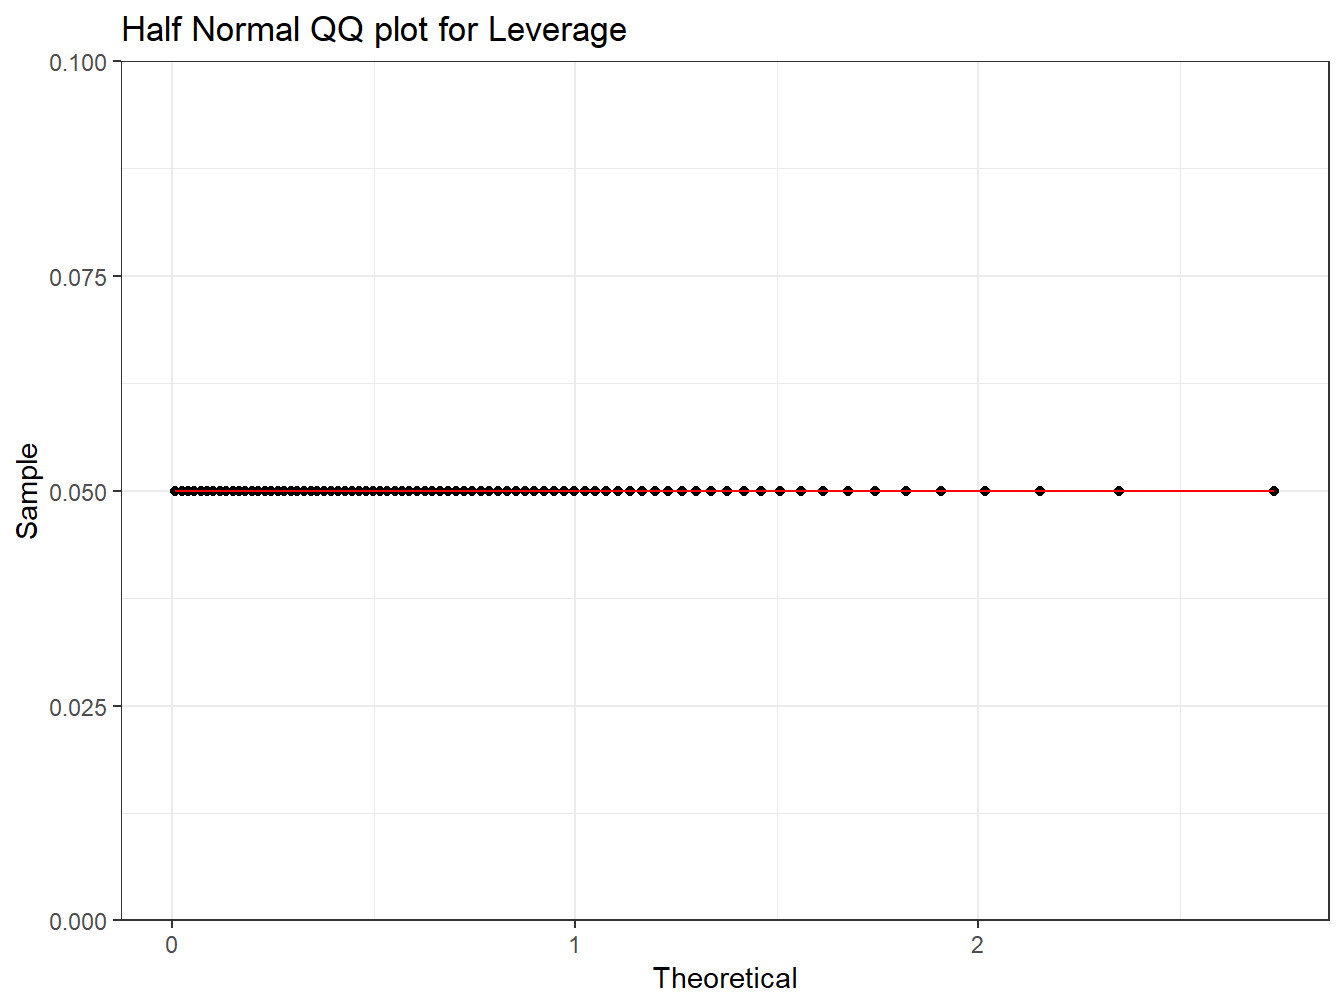
\includegraphics[width=0.8\linewidth]{final_exam_2_files/figure-latex/leverage-q4-1} 

}

\caption{Searching for highly influential points on the model}\label{fig:leverage-q4}
\end{figure}

Next we look for any highly irregular points used cooks distance. In Figure \ref{fig:cooks-q4} we can see that there are small deviations from the half normal expected quantiles. However, the scale of the graph is very small and so there are no points that I will examine furthur.

\begin{figure}

{\centering 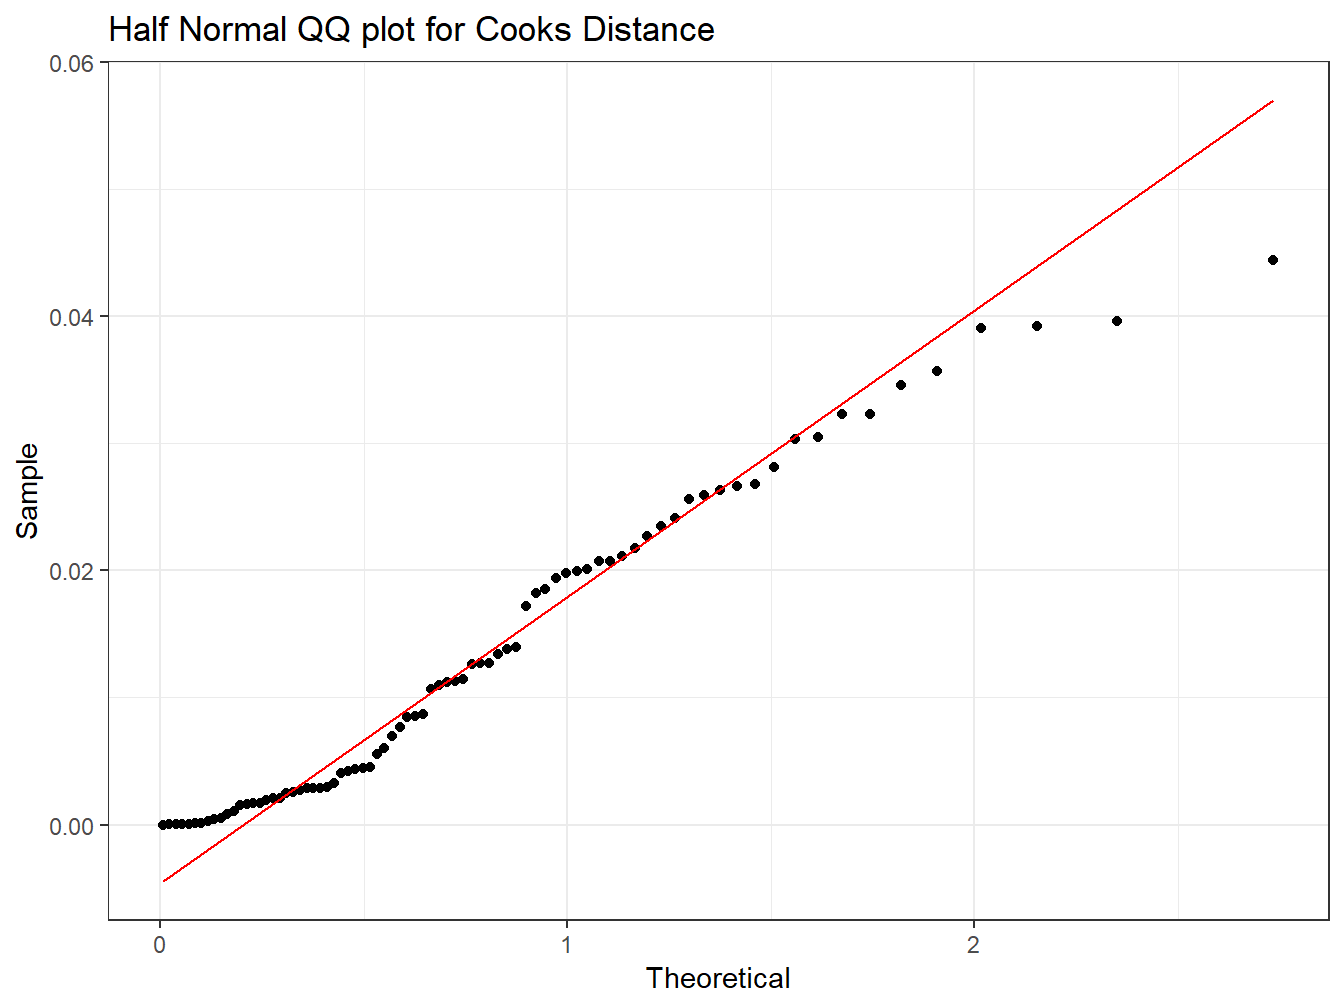
\includegraphics[width=0.8\linewidth]{final_exam_2_files/figure-latex/cooks-q4-1} 

}

\caption{Searching for irregular points}\label{fig:cooks-q4}
\end{figure}

\hypertarget{errors-1}{%
\subsection{Errors}\label{errors-1}}

Next I will check for constant variance in the residuals using the Residuals vs Fitted plot in Figure \ref{fig:resid-fit-q4}. There is nothing in the graph that leads me to believe that the variance is not consistent across the fitted values.

\begin{figure}

{\centering 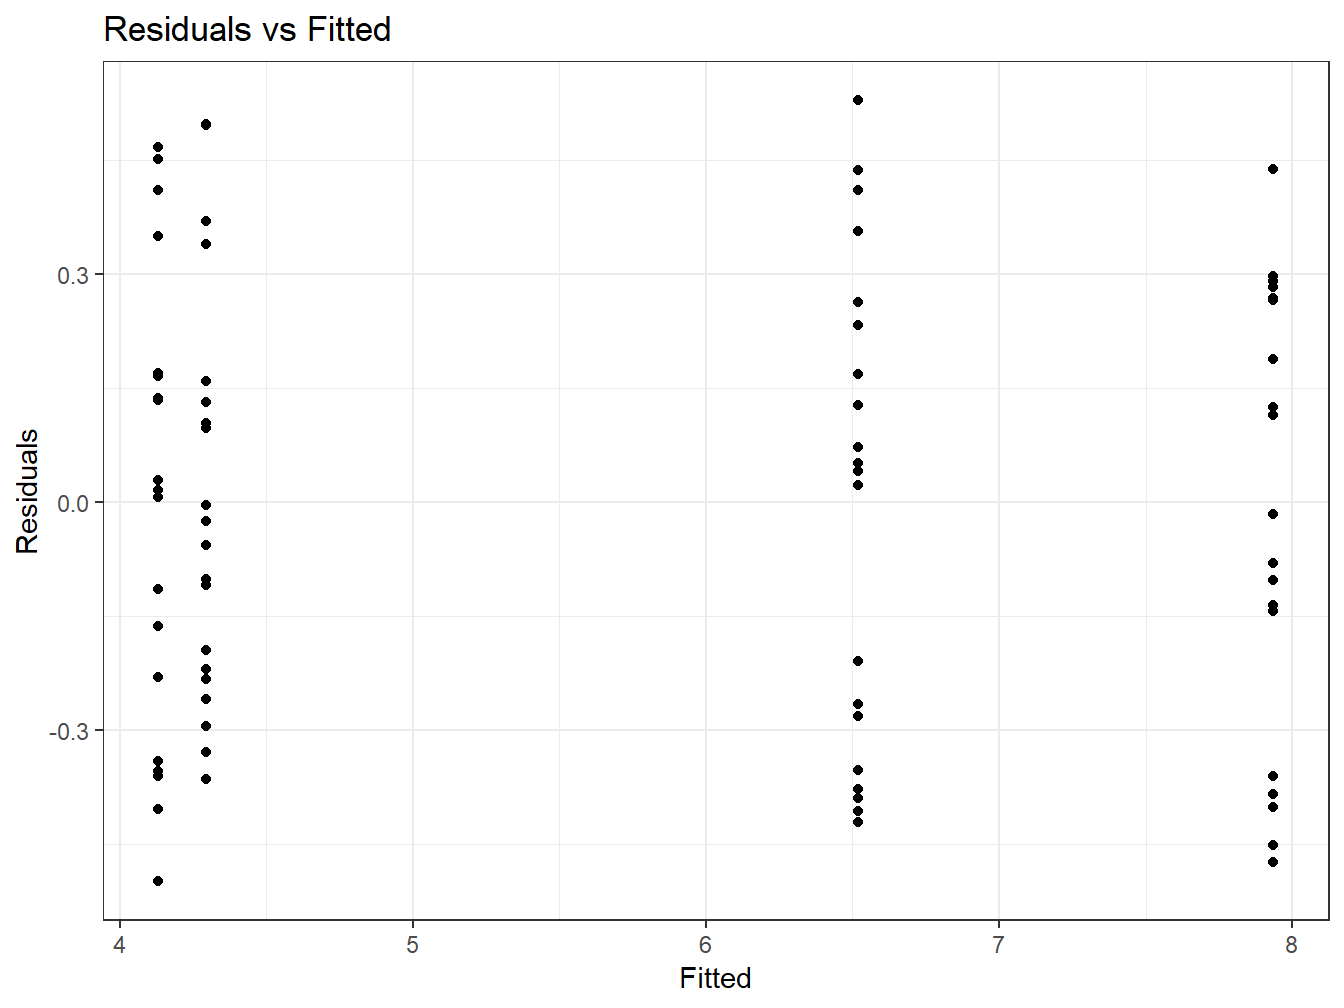
\includegraphics[width=0.8\linewidth]{final_exam_2_files/figure-latex/resid-fit-q4-1} 

}

\caption{Looking for non-constant variance}\label{fig:resid-fit-q4}
\end{figure}

Now I will check the normality of the residuals. In Figure \ref{fig:qq-norm-q4} the distribution looks very flat, possibly uniform.

\begin{figure}

{\centering 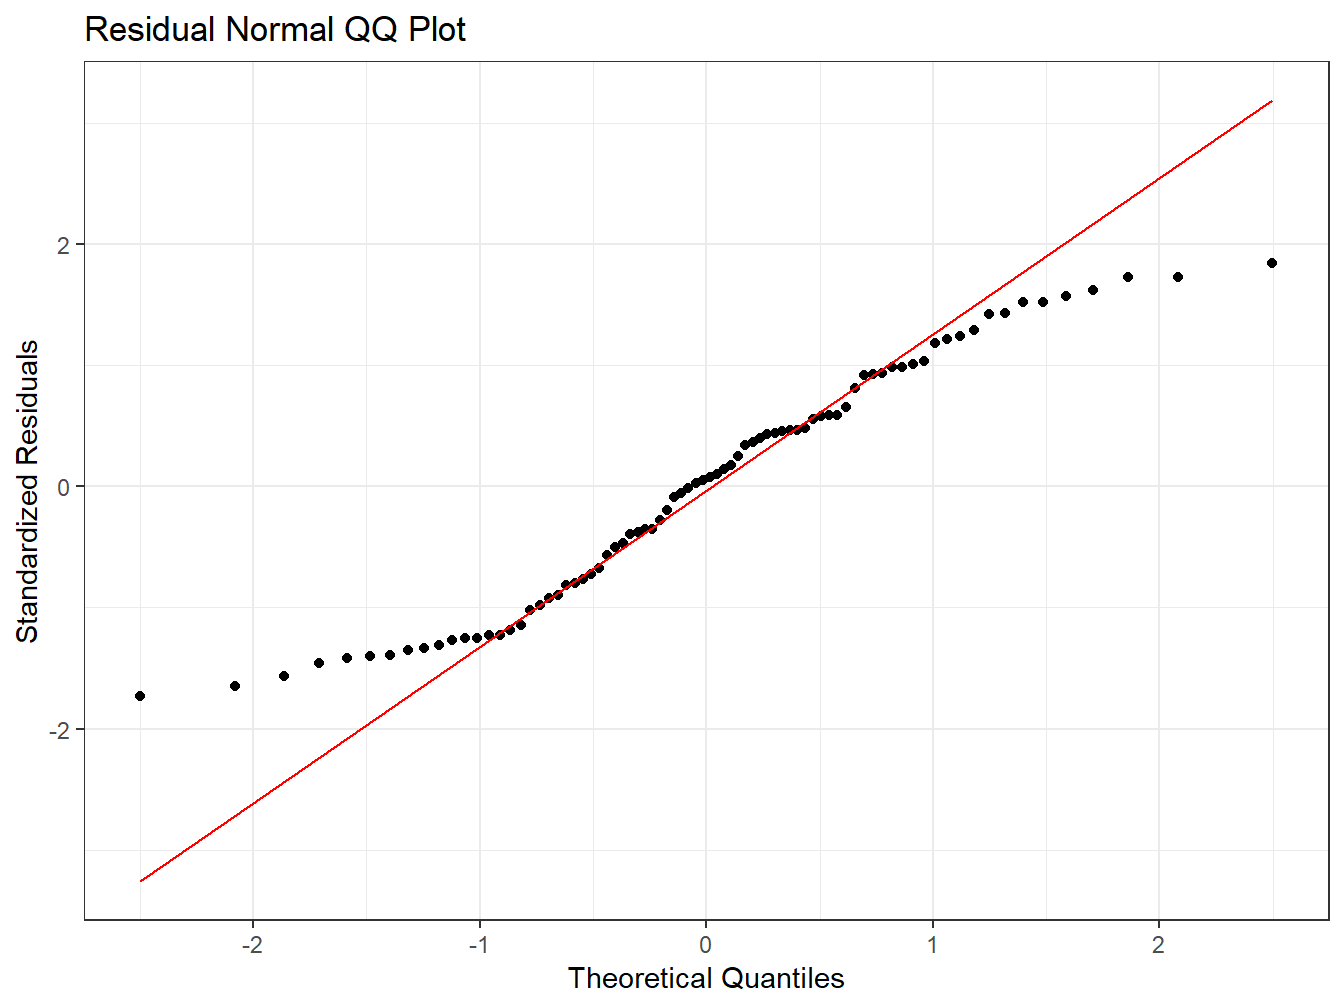
\includegraphics[width=0.8\linewidth]{final_exam_2_files/figure-latex/qq-norm-q4-1} 

}

\caption{Normal QQ plot for residuals}\label{fig:qq-norm-q4}
\end{figure}

In fact if we plot the Uniform(-1, 1) qq plot (like in Figure \ref{fig:qq-unif-q4}) we can see that the residuals probably do follow a uniform distribution. I think that the model assumption can still be approximately satisfied.

\begin{figure}

{\centering 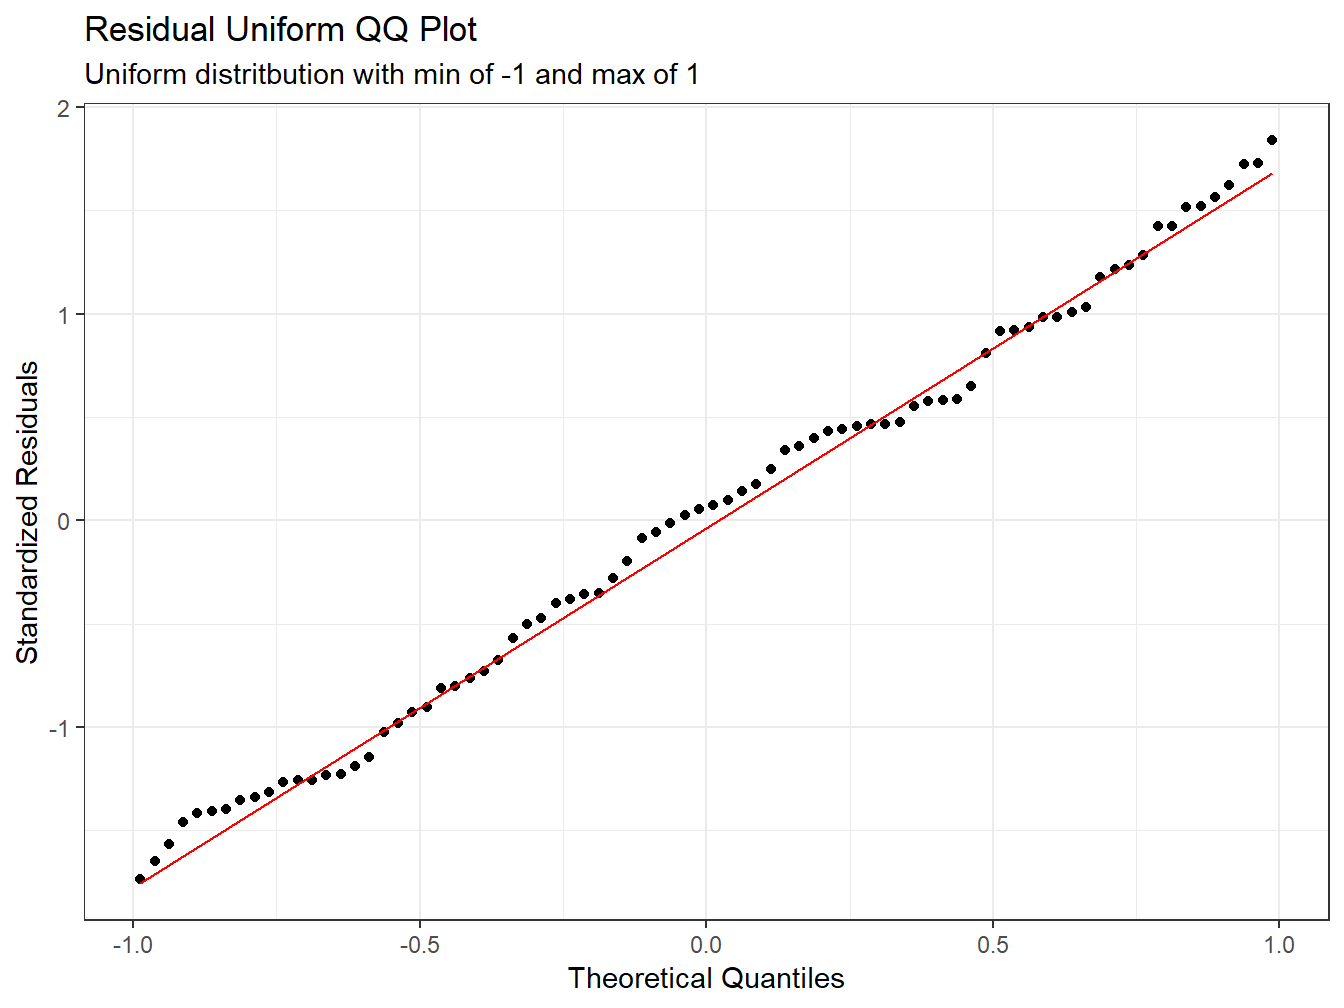
\includegraphics[width=0.8\linewidth]{final_exam_2_files/figure-latex/qq-unif-q4-1} 

}

\caption{Uniform QQ plot for residuals}\label{fig:qq-unif-q4}
\end{figure}

Finally, we do not have access to the researchers to ask them questions about the data collection process so the only check for independence amongst the residuals that I will do will be to plot the residuals in the order that they were reported in the text file to make sure there is no autocorrelation. This is done in Figure \ref{fig:resid-order-q4}

\begin{figure}

{\centering 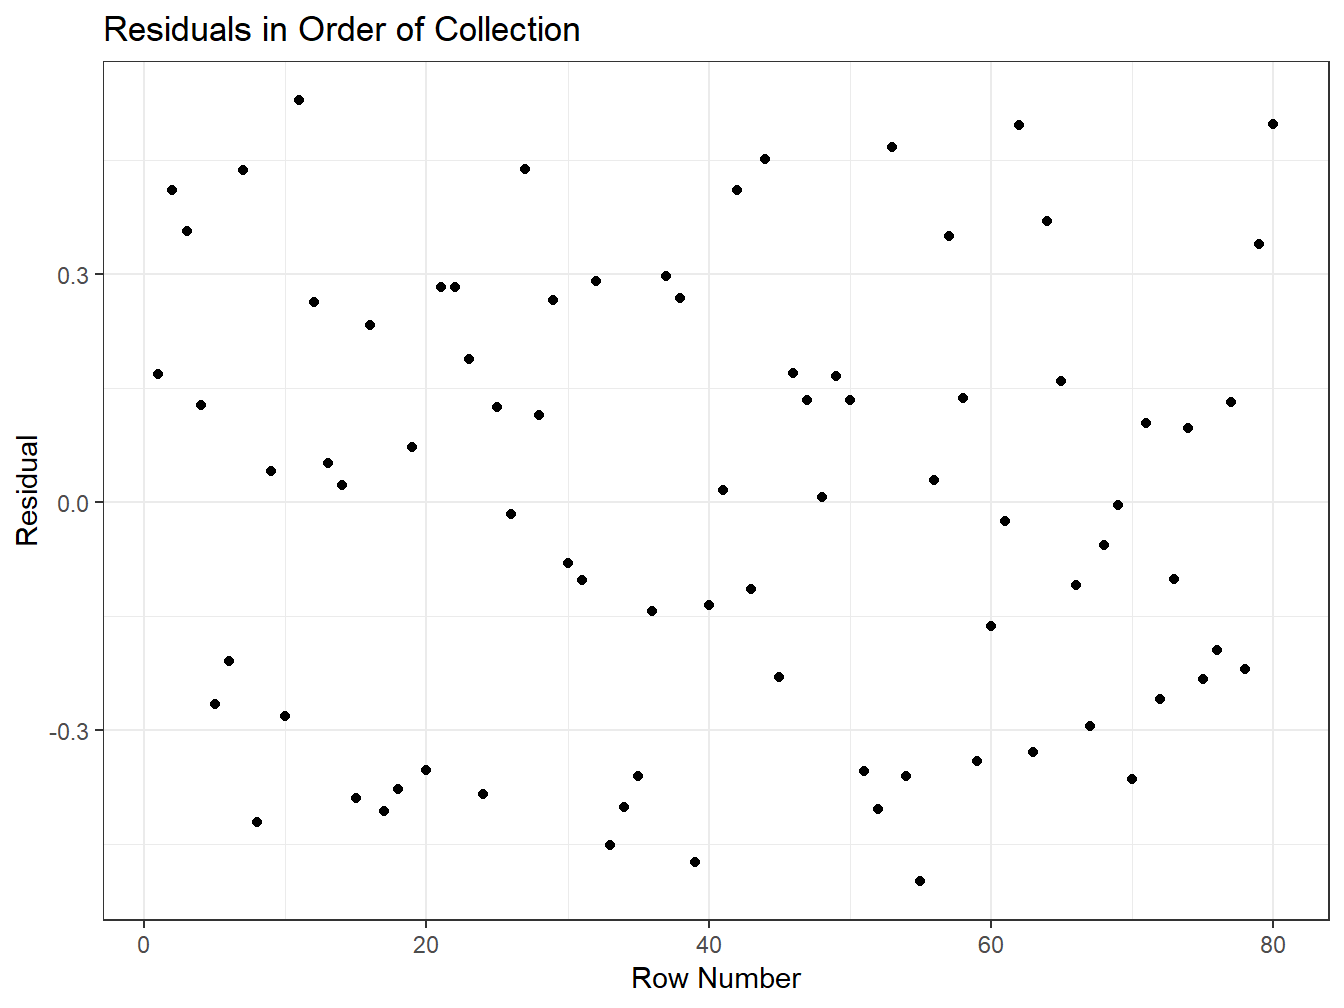
\includegraphics[width=0.8\linewidth]{final_exam_2_files/figure-latex/resid-order-q4-1} 

}

\caption{Independence of Order Reported}\label{fig:resid-order-q4}
\end{figure}

Overall, I do not think that any of the assumptions are not at least approximately satisified. I believe it is important to note that the residuals look to be uniformly distributed but that it does not change our inferences.

\hypertarget{part-e-2}{%
\section{Part E}\label{part-e-2}}

If I had a balanced expereiment with no interaction between the factors and I was searching for an difference in means of 1 unit or more that can be detected 80\% of the time with significance level 0.05 then I could run a power analysis to determine the sample size needed.

Since we are assuming there is no interaction between factors we can treat this like 2 independent 2 sample t tests. The power anlaysis to determine the sample size needed in a 2 sample t test depends on the alpha level (0.05), the power (0.80), the effect size (1) and the pooled standard deviation (not given in the question).

For impurity, the pooled standard deviation for the two groups is 0.5875189 and for density the pooled standard deviation for the two groups is 1.5854313. With these values we can compute the sample size needed for one group in each case independently. We can then take the larger of the two values as the sample size needed for one group. We can multiply that value by 2 to get the total sample size we need.

To calculate the sample size needed for one group in each caes I used the following formula

\begin{align}
  n_{\text{var}} &= \bigg( \sigma_{\text{var}} (z_{0.975} + z_{0.80} ) / 1 \bigg)^2
\end{align}

For impurity the sample size needed for one group is 6 and for density it is 40. The bigger of the two is 40 so 80 is the total sample size needed for the experiment.

\hypertarget{question-5}{%
\chapter{Question 5}\label{question-5}}

\hypertarget{part-a-4}{%
\section{Part A}\label{part-a-4}}

This experimental design is called Latin Squares since each treatment is assigned to each block once and only once and there are two blocking variables each with the same amount of levels (4) which is also equal to the number of treatments.

\hypertarget{part-b-4}{%
\section{Part B}\label{part-b-4}}

I made two plots (Figure \ref{fig:plots-fct-q5}) to investigate the effect of the blocking factors and the treatment on sales. Since we have such little data it is hard to tell if there is an effect or interactions between the blocking factors and treatment. With this data there seems to be interactions between the blocking factors and the treatment.

\begin{figure}

{\centering 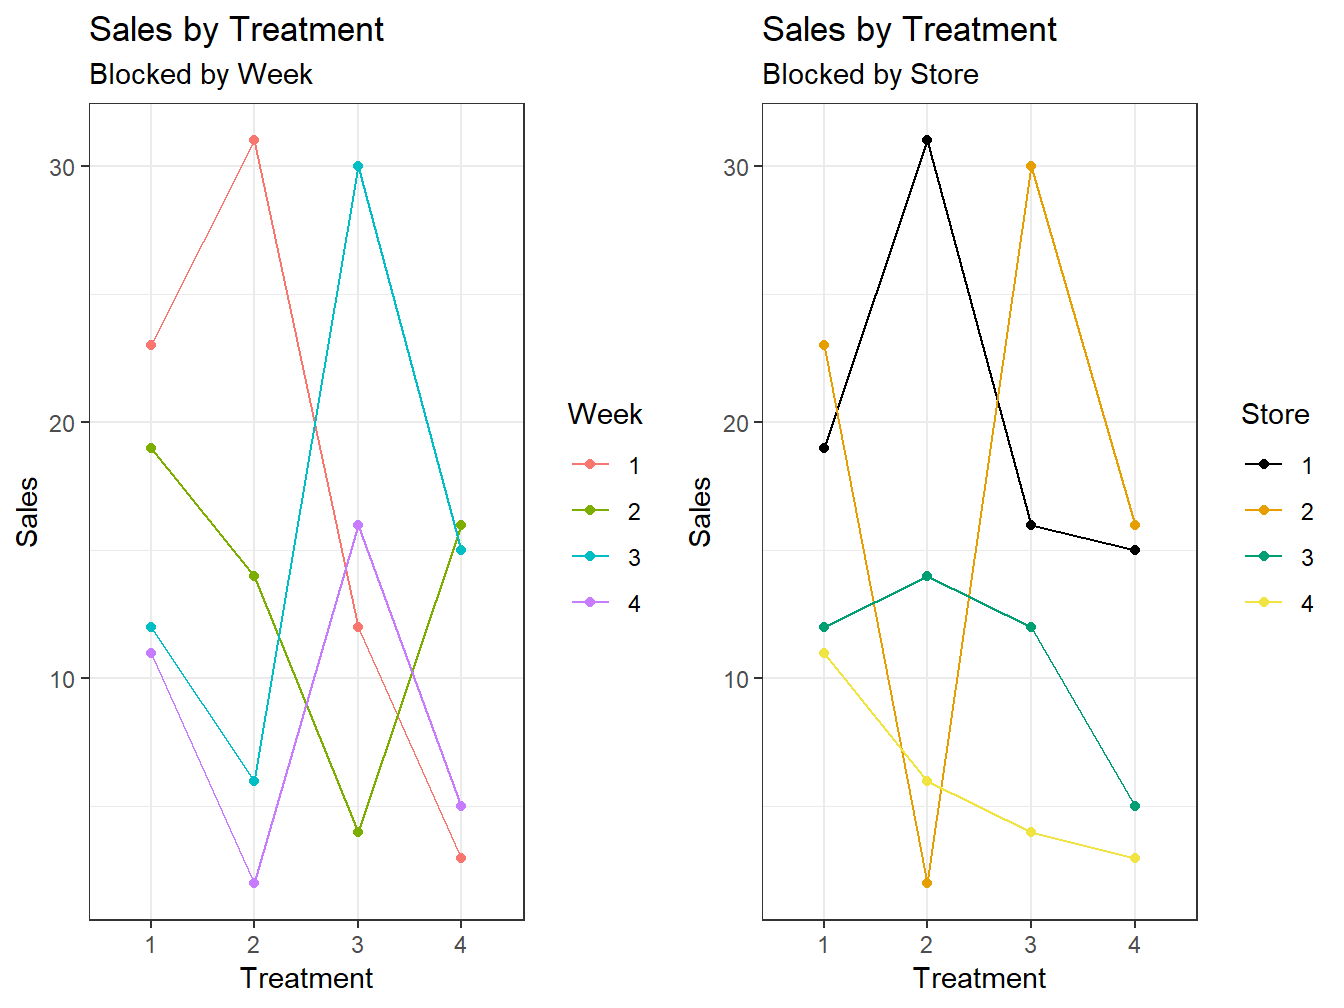
\includegraphics[width=0.8\linewidth]{final_exam_2_files/figure-latex/plots-fct-q5-1} 

}

\caption{Investigating effect of blocking factors and treatment on sales}\label{fig:plots-fct-q5}
\end{figure}

\hypertarget{part-c-4}{%
\section{Part C}\label{part-c-4}}

We cannot estimate interactions in the Latin Square so an appropriate model would be

\begin{align}
  y_{h, i, j} &= \mu + \alpha_h + \beta_i + \delta_j + \epsilon_{h, i, j}
\end{align}

where \(h = 1, 2, 3, 4\) is the week number, \(i = 1, 2, 3, 4\) is the store number and \(j = 1, 2, 3, 4\) is the treatment number. \(\epsilon \sim N(0, \sigma^2)\). We have to assume that the treatment and two blocking factors do not interact. Note that the \(\mu\) is a basleline with the first level of each blocking factor and treatment absorbed in. There is an argument to be made to treat week as a random effect and a smaller case to treat store as a random effect (if there are other stores that we care about we should), however, I have not done so here.

The estimated parameters for the described model are shown in Table \ref{tab:param-est-q5}.

\begin{table}

\caption{\label{tab:param-est-q5}Model coefficients}
\centering
\begin{tabular}[t]{lr}
\toprule
Term & Estimate\\
\midrule
Intercept & 26.38\\
Treatment2 & -3.00\\
Treatment3 & -0.75\\
Treatment4 & -6.50\\
Week2 & -4.00\\
\addlinespace
Week3 & -1.50\\
Week4 & -8.75\\
Store2 & -2.50\\
Store3 & -9.50\\
Store4 & -14.25\\
\bottomrule
\end{tabular}
\end{table}

\hypertarget{part-d-4}{%
\section{Part D}\label{part-d-4}}

Similarily to \protect\hyperlink{question-2}{Question 2} and \protect\hyperlink{question-4}{Question 4} I will check for influential outliers and those that seem like they not belong, I will check for equal variance, normality, and independence amongst the residuals. We have assumed also here that there is no interactions between the regressors. We saw in the initial plot that this may not be exactly the case.

\hypertarget{outliers-2}{%
\subsection{Outliers}\label{outliers-2}}

Like in \protect\hyperlink{question-4}{Question 4} due to the design all the points have the same leverage. Therefore Figure \ref{fig:lev-q5} is not very interesting.

\begin{figure}

{\centering 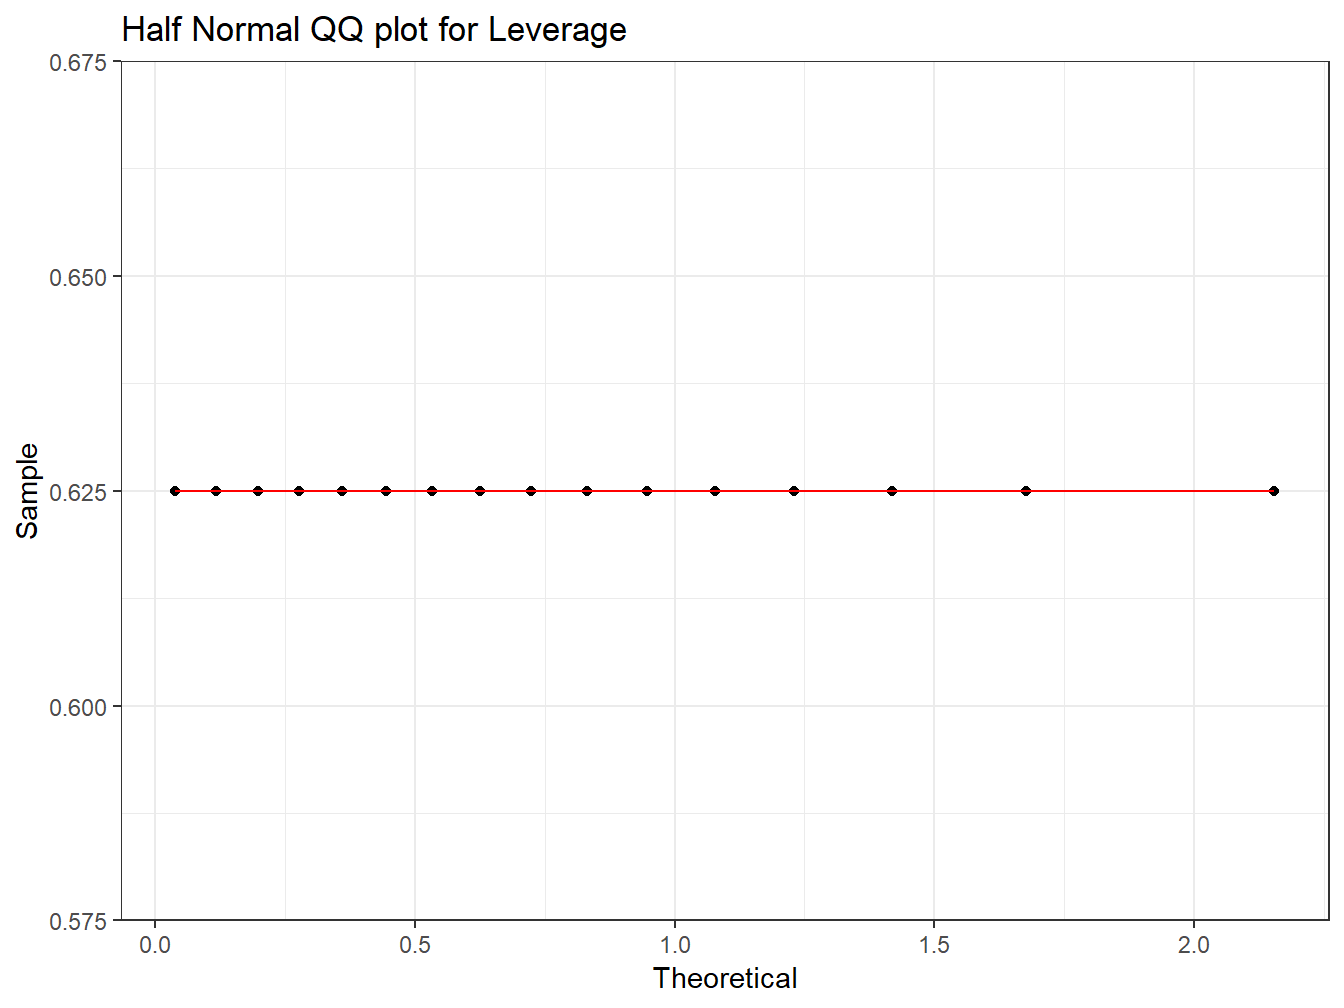
\includegraphics[width=0.8\linewidth]{final_exam_2_files/figure-latex/lev-q5-1} 

}

\caption{Searching for influential points on the model}\label{fig:lev-q5}
\end{figure}

There are some very large outliers as can be seen in \ref{fig:cooks-q5}. This may be because we have not accounted for interactions between regressors. However, there is no real action to take since we have such little data.

\begin{figure}

{\centering 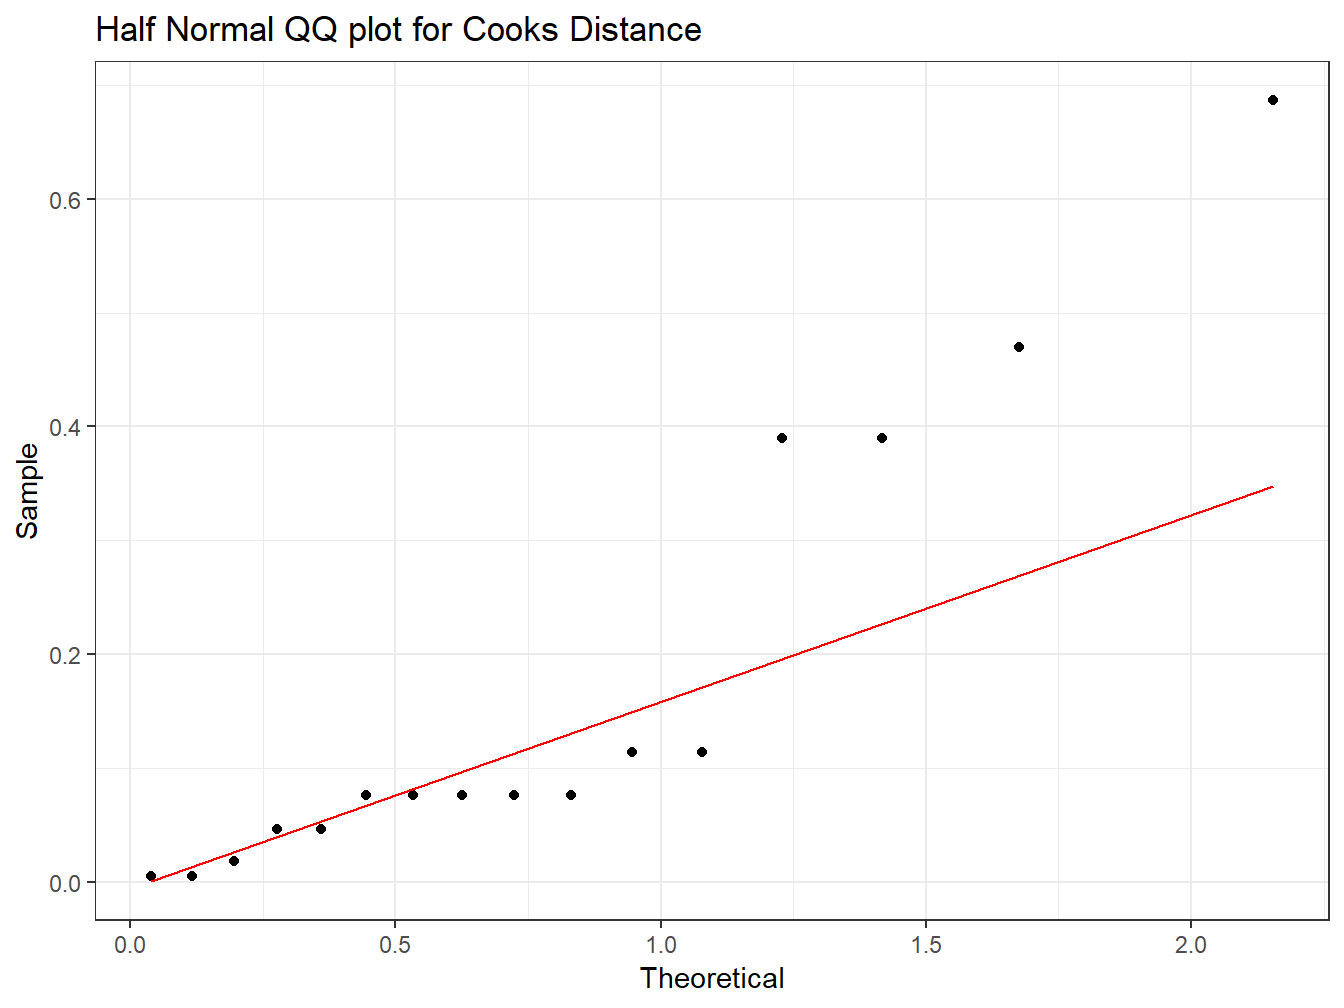
\includegraphics[width=0.8\linewidth]{final_exam_2_files/figure-latex/cooks-q5-1} 

}

\caption{Searching for Outliers}\label{fig:cooks-q5}
\end{figure}

\hypertarget{resiudals}{%
\subsection{Resiudals}\label{resiudals}}

Since we have such few points it is tough to see if there is any non-constant variance in the residuals. However, with what we have in Figure \ref{fig:resid-fit-q5} I think this is a safe assumption.

\begin{figure}

{\centering 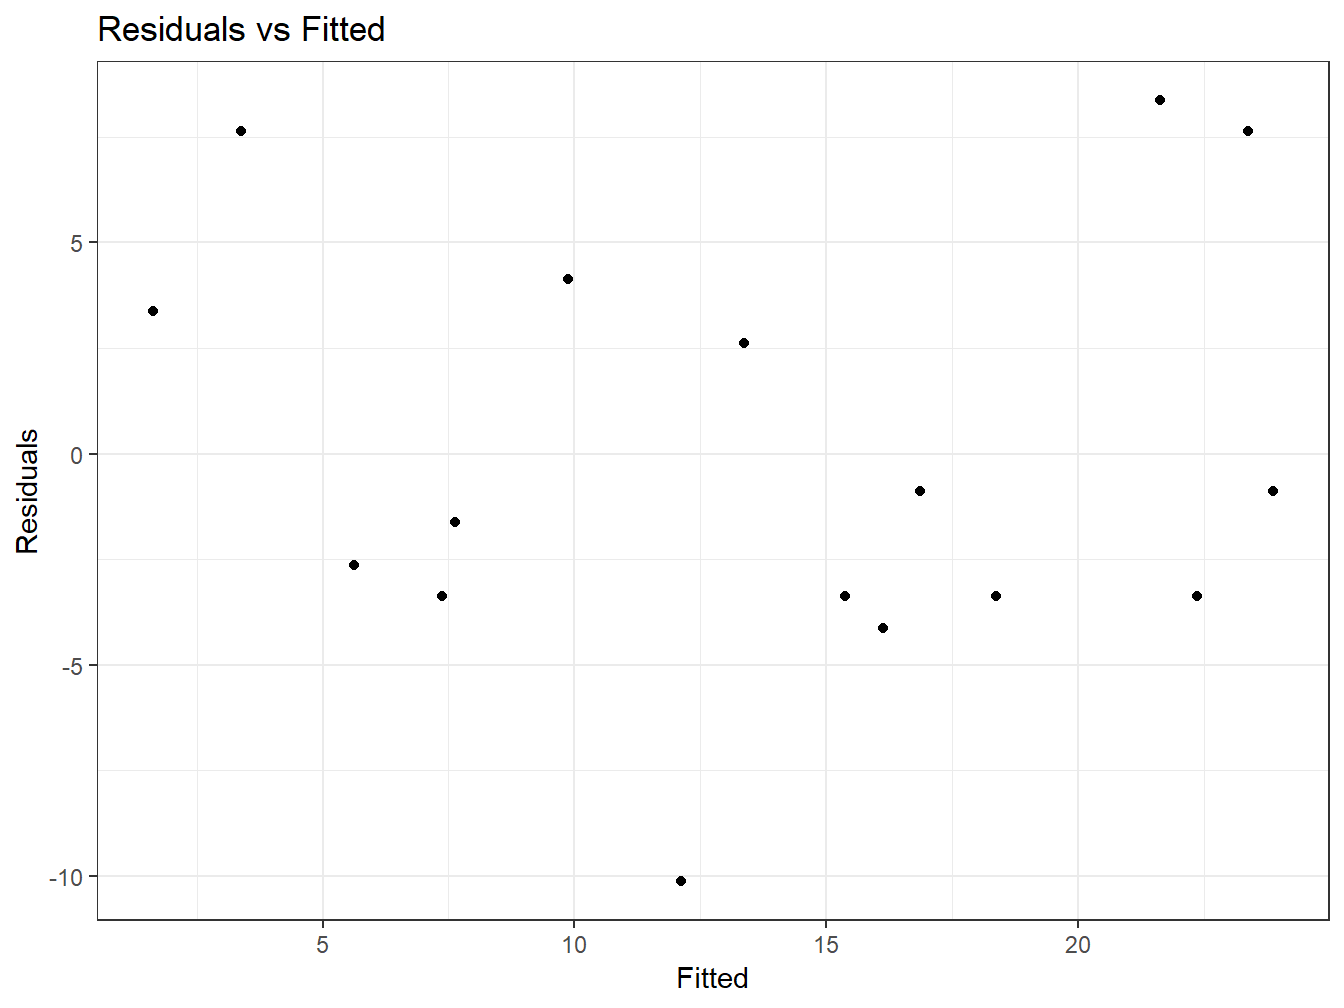
\includegraphics[width=0.8\linewidth]{final_exam_2_files/figure-latex/resid-fit-q5-1} 

}

\caption{Looking for Non-Constant Variance}\label{fig:resid-fit-q5}
\end{figure}

With only 16 points I do not see enough evidence to believe that the residuals are not normal when looking at Figure \ref{fig:qq-q5}.

\begin{figure}

{\centering 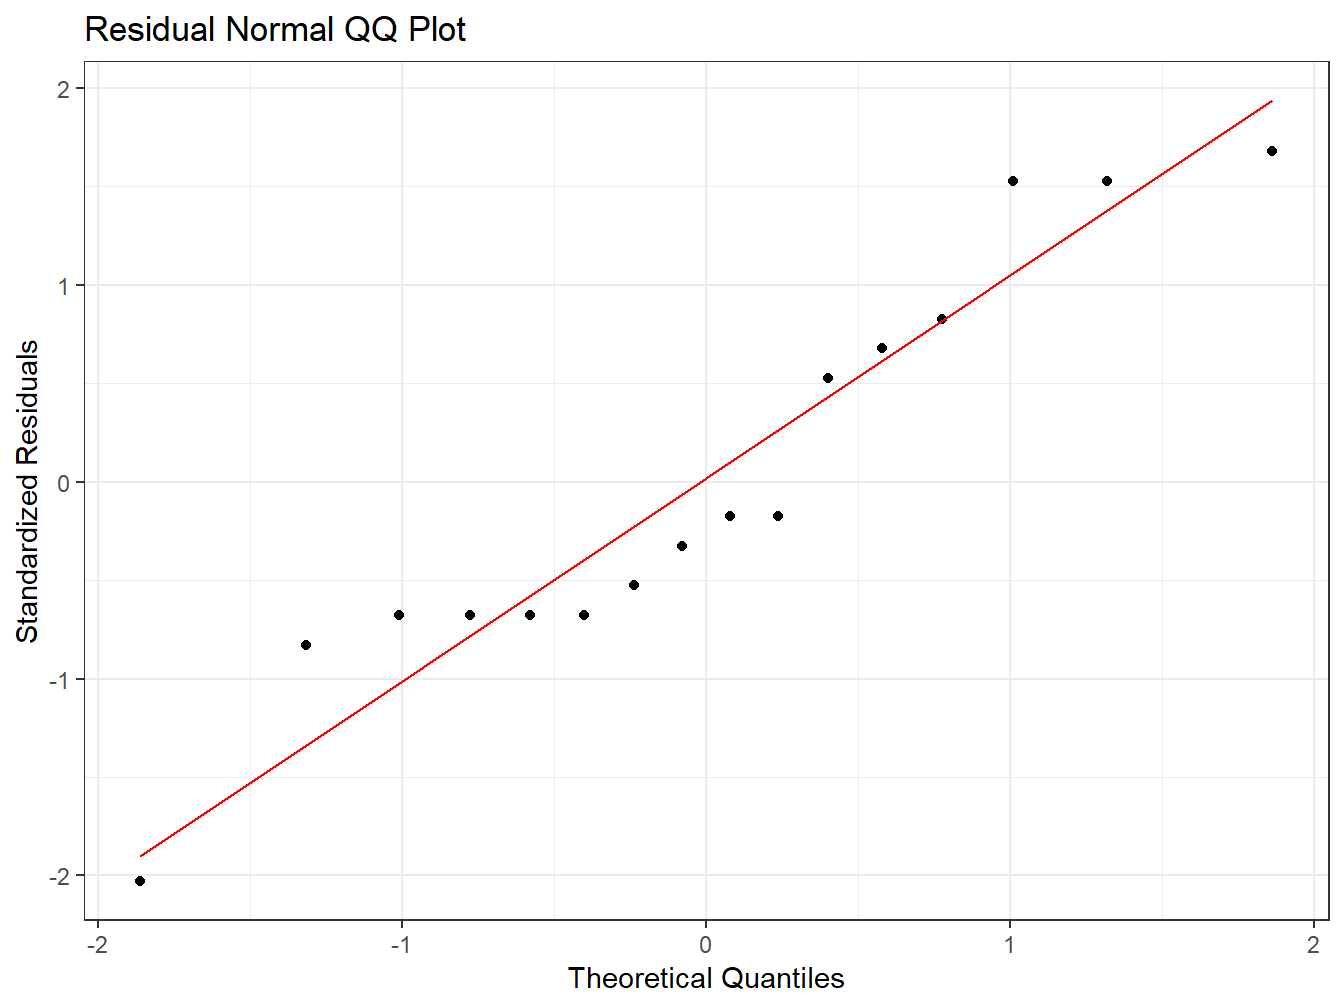
\includegraphics[width=0.8\linewidth]{final_exam_2_files/figure-latex/qq-q5-1} 

}

\caption{Are the residuals normal}\label{fig:qq-q5}
\end{figure}

Finally, I check in Figure \ref{fig:order-q5} if there is an effect based on the order the data was collected. I do not see anything to indicate theres anything wrong.

\begin{figure}

{\centering 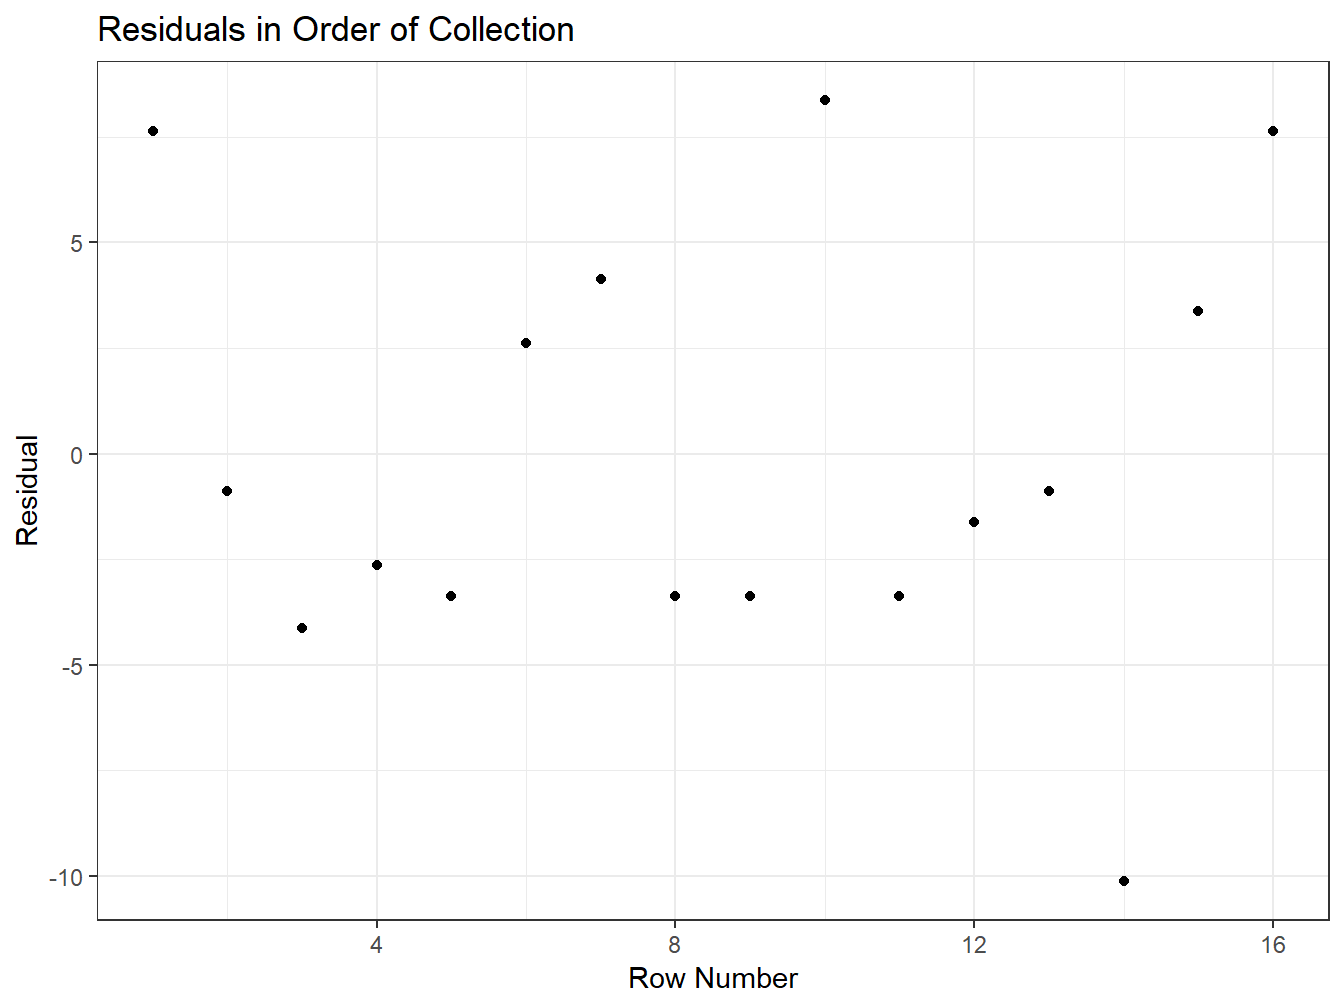
\includegraphics[width=0.8\linewidth]{final_exam_2_files/figure-latex/order-q5-1} 

}

\caption{Order of Collection}\label{fig:order-q5}
\end{figure}

\hypertarget{part-e-3}{%
\section{Part E}\label{part-e-3}}

I will test to see if there is an effect of treatment on sales. I will do so by taking the null hypothesis that \(\text{treatment}_1 = \text{treatment}_2 = \text{treatment}_3 = \text{treatment}_4 = 0\). For the alternative that atleast one of the effects is not equal to 0. The test statisitc follows an \(F\) distribution. The results are displayed in Table \ref{tab:test-q5}. Since the p value is greater than \(0.05\) we will fail to reject the null hypothesis. Of course this is not terribly surprising considering the small size of the data set.

\begin{table}

\caption{\label{tab:test-q5}Test for the effect of Treatment on Sales}
\centering
\begin{tabular}[t]{lrr}
\toprule
Term & Statistic & P Value\\
\midrule
Treatment & 0.51 & 0.69\\
\bottomrule
\end{tabular}
\end{table}

\hypertarget{part-f-2}{%
\section{Part F}\label{part-f-2}}

The model I would propose would be,

\begin{align}
  y_{h, i, j} &= \mu + \alpha_h + \beta_{i} + \delta_j + \epsilon_{h, i, j}
\end{align}

W
where \(h = 1, 2, 3, 4, 5, 6, 7, 8\) is the week number, \(i = 1, 2, 3, 4, 5, 6, 7, 8\) is the store number and \(j = 1, 2, 3, 4\) is the treatment number. \(\epsilon \sim N(0, \sigma^2)\).

\bibliography{book.bib,packages.bib}


\end{document}
